\documentclass[letterpaper]{book}
\usepackage{makeidx}
\usepackage{graphicx}
\usepackage{multicol}
\usepackage{float}
\usepackage{listings}
\usepackage{color}
\usepackage{ifthen}
\usepackage[table]{xcolor}
\usepackage{textcomp}
\usepackage{alltt}
\usepackage{ifpdf}
\ifpdf
\usepackage[pdftex,
            pagebackref=true,
            colorlinks=true,
            linkcolor=blue,
            unicode
           ]{hyperref}
\else
\usepackage[ps2pdf,
            pagebackref=true,
            colorlinks=true,
            linkcolor=blue,
            unicode
           ]{hyperref}
\usepackage{pspicture}
\fi
\usepackage[utf8]{inputenc}
\usepackage{mathptmx}
\usepackage[scaled=.90]{helvet}
\usepackage{courier}
\usepackage{doxygen}
\lstset{language=C++,inputencoding=utf8,basicstyle=\footnotesize,breaklines=true,breakatwhitespace=true,tabsize=8,numbers=left }
\makeindex
\setcounter{tocdepth}{3}
\renewcommand{\footrulewidth}{0.4pt}
\begin{document}
\hypersetup{pageanchor=false}
\begin{titlepage}
\vspace*{7cm}
\begin{center}
{\Large ebf }\\
\vspace*{1cm}
{\large Generated by Doxygen 1.7.3}\\
\vspace*{0.5cm}
{\small Wed Aug 22 2012 10:38:11}\\
\end{center}
\end{titlepage}
\clearemptydoublepage
\pagenumbering{roman}
\tableofcontents
\clearemptydoublepage
\pagenumbering{arabic}
\hypersetup{pageanchor=true}
\chapter{Directory Hierarchy}
\section{Directories}
This directory hierarchy is sorted roughly, but not completely, alphabetically:\begin{DoxyCompactList}
\item \contentsline{section}{src}{\pageref{dir_703a5f36a5fc7abb67197856d62eb3e4}}{}
\end{DoxyCompactList}

\chapter{Namespace Index}
\section{Namespace List}
Here is a list of all namespaces with brief descriptions:\begin{DoxyCompactList}
\item\contentsline{section}{\hyperlink{namespacedbconfig}{dbconfig} }{\pageref{namespacedbconfig}}{}
\item\contentsline{section}{\hyperlink{namespaceebf}{ebf} (Created on Jun 19, 2012 )}{\pageref{namespaceebf}}{}
\item\contentsline{section}{\hyperlink{namespacefunctions}{functions} }{\pageref{namespacefunctions}}{}
\item\contentsline{section}{\hyperlink{namespacemakeblc}{makeblc} }{\pageref{namespacemakeblc}}{}
\item\contentsline{section}{\hyperlink{namespacemakeplc}{makeplc} }{\pageref{namespacemakeplc}}{}
\item\contentsline{section}{\hyperlink{namespacemlp}{mlp} }{\pageref{namespacemlp}}{}
\item\contentsline{section}{\hyperlink{namespacerunpoly}{runpoly} (Created on Jul 2, 2012 )}{\pageref{namespacerunpoly}}{}
\item\contentsline{section}{\hyperlink{namespacerunpoly__dan__6}{runpoly\_\-dan\_\-6} }{\pageref{namespacerunpoly__dan__6}}{}
\item\contentsline{section}{\hyperlink{namespaceruntrained}{runtrained} (Created on Jul 6, 2012 )}{\pageref{namespaceruntrained}}{}
\item\contentsline{section}{\hyperlink{namespacetrainnet}{trainnet} (Created on Jul 5, 2012 )}{\pageref{namespacetrainnet}}{}
\item\contentsline{section}{\hyperlink{namespacetrainnetmp}{trainnetmp} (Created on Jul 18, 2012 )}{\pageref{namespacetrainnetmp}}{}
\end{DoxyCompactList}

\chapter{Class Index}
\section{Class Hierarchy}
This inheritance list is sorted roughly, but not completely, alphabetically:\begin{DoxyCompactList}
\item \contentsline{section}{Exception}{\pageref{classException}}{}
\begin{DoxyCompactList}
\item \contentsline{section}{mlp::MlpError}{\pageref{classmlp_1_1MlpError}}{}
\end{DoxyCompactList}
\item \contentsline{section}{object}{\pageref{classobject}}{}
\begin{DoxyCompactList}
\item \contentsline{section}{dbconfig::Asas}{\pageref{classdbconfig_1_1Asas}}{}
\item \contentsline{section}{mlp::mlp}{\pageref{classmlp_1_1mlp}}{}
\end{DoxyCompactList}
\end{DoxyCompactList}

\chapter{Class Index}
\section{Class List}
Here are the classes, structs, unions and interfaces with brief descriptions:\begin{DoxyCompactList}
\item\contentsline{section}{\hyperlink{classdbconfig_1_1Asas}{dbconfig::Asas} (Class wrapper for ASAS column definitions, types etc )}{\pageref{classdbconfig_1_1Asas}}{}
\item\contentsline{section}{\hyperlink{classException}{Exception} }{\pageref{classException}}{}
\item\contentsline{section}{\hyperlink{classmlp_1_1mlp}{mlp::mlp} (A Multi-\/Layer Perceptron )}{\pageref{classmlp_1_1mlp}}{}
\item\contentsline{section}{\hyperlink{classmlp_1_1MlpError}{mlp::MlpError} (\hyperlink{classException}{Exception} class for mlp )}{\pageref{classmlp_1_1MlpError}}{}
\item\contentsline{section}{\hyperlink{classobject}{object} }{\pageref{classobject}}{}
\end{DoxyCompactList}

\chapter{File Index}
\section{File List}
Here is a list of all files with brief descriptions:\begin{DoxyCompactList}
\item\contentsline{section}{src/\hyperlink{dbconfig_8py}{dbconfig.py} }{\pageref{dbconfig_8py}}{}
\item\contentsline{section}{src/\hyperlink{functions_8py}{functions.py} }{\pageref{functions_8py}}{}
\item\contentsline{section}{src/\hyperlink{makeblc_8py}{makeblc.py} }{\pageref{makeblc_8py}}{}
\item\contentsline{section}{src/\hyperlink{makeplc_8py}{makeplc.py} }{\pageref{makeplc_8py}}{}
\item\contentsline{section}{src/\hyperlink{mlp_8py}{mlp.py} }{\pageref{mlp_8py}}{}
\item\contentsline{section}{src/\hyperlink{runpoly_8py}{runpoly.py} }{\pageref{runpoly_8py}}{}
\item\contentsline{section}{src/\hyperlink{runpoly__dan__6_8py}{runpoly\_\-dan\_\-6.py} }{\pageref{runpoly__dan__6_8py}}{}
\item\contentsline{section}{src/\hyperlink{runtrained_8py}{runtrained.py} }{\pageref{runtrained_8py}}{}
\item\contentsline{section}{src/\hyperlink{trainnet_8py}{trainnet.py} }{\pageref{trainnet_8py}}{}
\item\contentsline{section}{src/\hyperlink{trainnetmp_8py}{trainnetmp.py} }{\pageref{trainnetmp_8py}}{}
\end{DoxyCompactList}

\chapter{Directory Documentation}
\hypertarget{dir_703a5f36a5fc7abb67197856d62eb3e4}{
\section{src/ Directory Reference}
\label{dir_703a5f36a5fc7abb67197856d62eb3e4}\index{src/ Directory Reference@{src/ Directory Reference}}
}
Directory dependency graph for src/:\nopagebreak
\begin{figure}[H]
\begin{center}
\leavevmode
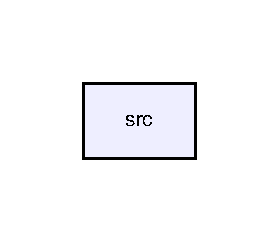
\includegraphics[width=134pt]{dir_703a5f36a5fc7abb67197856d62eb3e4_dep}
\end{center}
\end{figure}
\subsection*{Files}
\begin{DoxyCompactItemize}
\item 
file \hyperlink{dbconfig_8py}{dbconfig.py}
\item 
file \hyperlink{functions_8py}{functions.py}
\item 
file \hyperlink{makeblc_8py}{makeblc.py}
\item 
file \hyperlink{makeplc_8py}{makeplc.py}
\item 
file \hyperlink{mlp_8py}{mlp.py}
\item 
file \hyperlink{plotlc_8py}{plotlc.py}
\item 
file \hyperlink{runpoly_8py}{runpoly.py}
\item 
file \hyperlink{runpoly__dan__6_8py}{runpoly\_\-dan\_\-6.py}
\item 
file \hyperlink{runpolymp_8py}{runpolymp.py}
\item 
file \hyperlink{runtrained_8py}{runtrained.py}
\item 
file \hyperlink{trainnet_8py}{trainnet.py}
\item 
file \hyperlink{trainnetmp_8py}{trainnetmp.py}
\end{DoxyCompactItemize}

\chapter{Namespace Documentation}
\hypertarget{namespacedbconfig}{
\section{dbconfig Namespace Reference}
\label{namespacedbconfig}\index{dbconfig@{dbconfig}}
}
\subsection*{Classes}
\begin{DoxyCompactItemize}
\item 
class \hyperlink{classdbconfig_1_1Asas}{Asas}
\begin{DoxyCompactList}\small\item\em class wrapper for ASAS column definitions, types etc \item\end{DoxyCompactList}\end{DoxyCompactItemize}

\hypertarget{namespaceebf}{
\section{ebf Namespace Reference}
\label{namespaceebf}\index{ebf@{ebf}}
}


Created on Jun 19, 2012.  




\subsection{Detailed Description}
Created on Jun 19, 2012. Created on Jun 28, 2012.

Created on Jun 18, 2012.

\begin{DoxyAuthor}{Author}
mpaegert 
\end{DoxyAuthor}
\begin{DoxyVersion}{Version}
\$Revision: 1.2 $ 
\end{DoxyVersion}
\begin{DoxyDate}{Date}
\$Date: 2012/08/22 15:45:53 $
\end{DoxyDate}
\begin{DoxyParagraph}{Log:}
\hyperlink{dbconfig_8py}{dbconfig.py},v 
\end{DoxyParagraph}
Revision 1.1 2012/07/06 20:34:19 paegerm Initial revision

Initial revision

\begin{DoxyAuthor}{Author}
mpaegert 
\end{DoxyAuthor}
\begin{DoxyVersion}{Version}
\$Revision: 1.2 $ 
\end{DoxyVersion}
\begin{DoxyDate}{Date}
\$Date: 2012/08/22 15:45:53 $
\end{DoxyDate}
\begin{DoxyParagraph}{Log:}
\hyperlink{functions_8py}{functions.py},v 
\end{DoxyParagraph}
Revision 1.1 2012/07/06 20:34:19 paegerm Initial revision

Initial revision

\begin{DoxyAuthor}{Author}
mpaegert 
\end{DoxyAuthor}
\begin{DoxyVersion}{Version}
\$Revision: 1.2 $ 
\end{DoxyVersion}
\begin{DoxyDate}{Date}
\$Date: 2012/08/22 15:45:53 $
\end{DoxyDate}
make phase folded light curves

\begin{DoxyParagraph}{Log:}
\hyperlink{makeblc_8py}{makeblc.py},v 
\end{DoxyParagraph}
Revision 1.1 2012/07/06 20:34:19 paegerm Initial revision

\begin{DoxyAuthor}{Author}
mpaegert 
\end{DoxyAuthor}
\begin{DoxyVersion}{Version}
\$Revision: 1.2 $ 
\end{DoxyVersion}
\begin{DoxyDate}{Date}
\$Date: 2012/08/22 15:45:53 $
\end{DoxyDate}
make phase folded light curves

\begin{DoxyParagraph}{Log:}
\hyperlink{makeplc_8py}{makeplc.py},v 
\end{DoxyParagraph}
Revision 1.1 2012/07/06 20:34:19 paegerm Initial revision

\begin{DoxyAuthor}{Author}
mpaegert 
\end{DoxyAuthor}
\begin{DoxyVersion}{Version}
\$Revision: 1.2 $ 
\end{DoxyVersion}
\begin{DoxyDate}{Date}
\$Date: 2012/08/22 15:45:53 $
\end{DoxyDate}
A simple muulti-\/layer perceptron, currently restricted to one hidden layer

: numpy

\begin{DoxyParagraph}{Log:}
\hyperlink{mlp_8py}{mlp.py},v 
\end{DoxyParagraph}
Revision 1.2 2012/07/20 20:22:22 paegerm $\ast$$\ast$$\ast$ empty log message $\ast$$\ast$$\ast$

Adding documentation, adding normalize option to evaluate(), adding stopval to earlystopping() Adding MlpError class

Revision 1.1 2012/07/06 20:34:19 paegerm Initial revision 
\hypertarget{namespacefunctions}{
\section{functions Namespace Reference}
\label{namespacefunctions}\index{functions@{functions}}
}
\subsection*{Functions}
\begin{DoxyCompactItemize}
\item 
def \hyperlink{namespacefunctions_ab417ff9b2580ed12b7937559adbc90f1}{makephasedlc}
\item 
def \hyperlink{namespacefunctions_a849aa559f687aad0e0cb251f83b4dc23}{deriv2}
\item 
def \hyperlink{namespacefunctions_a5cfda28c18921b966002c19c2b20b3e5}{makebinnedlc}
\end{DoxyCompactItemize}


\subsection{Function Documentation}
\hypertarget{namespacefunctions_a849aa559f687aad0e0cb251f83b4dc23}{
\index{functions@{functions}!deriv2@{deriv2}}
\index{deriv2@{deriv2}!functions@{functions}}
\subsubsection[{deriv2}]{\setlength{\rightskip}{0pt plus 5cm}def functions::deriv2 (
\begin{DoxyParamCaption}
\item[{}]{x, }
\item[{}]{y}
\end{DoxyParamCaption}
)}}
\label{namespacefunctions_a849aa559f687aad0e0cb251f83b4dc23}


Definition at line 40 of file functions.py.

\hypertarget{namespacefunctions_a5cfda28c18921b966002c19c2b20b3e5}{
\index{functions@{functions}!makebinnedlc@{makebinnedlc}}
\index{makebinnedlc@{makebinnedlc}!functions@{functions}}
\subsubsection[{makebinnedlc}]{\setlength{\rightskip}{0pt plus 5cm}def functions::makebinnedlc (
\begin{DoxyParamCaption}
\item[{}]{plc, }
\item[{}]{staruid, }
\item[{}]{nrbins = {\ttfamily 100}}
\end{DoxyParamCaption}
)}}
\label{namespacefunctions_a5cfda28c18921b966002c19c2b20b3e5}


Definition at line 53 of file functions.py.

\hypertarget{namespacefunctions_ab417ff9b2580ed12b7937559adbc90f1}{
\index{functions@{functions}!makephasedlc@{makephasedlc}}
\index{makephasedlc@{makephasedlc}!functions@{functions}}
\subsubsection[{makephasedlc}]{\setlength{\rightskip}{0pt plus 5cm}def functions::makephasedlc (
\begin{DoxyParamCaption}
\item[{}]{lc, }
\item[{}]{t0, }
\item[{}]{dictvmag, }
\item[{}]{period}
\end{DoxyParamCaption}
)}}
\label{namespacefunctions_ab417ff9b2580ed12b7937559adbc90f1}


Definition at line 21 of file functions.py.


\hypertarget{namespacemakeblc}{\section{makeblc Namespace Reference}
\label{namespacemakeblc}\index{makeblc@{makeblc}}
}

\hypertarget{namespacemakeplc}{
\section{makeplc Namespace Reference}
\label{namespacemakeplc}\index{makeplc@{makeplc}}
}
\subsection*{Variables}
\begin{DoxyCompactItemize}
\item 
string \hyperlink{namespacemakeplc_a9a367257ba494afb85e43b8b3330f85d}{usage} = '\%prog \mbox{[}options\mbox{]} plcdbfile'
\item 
tuple \hyperlink{namespacemakeplc_aab6ec9062bd8992b365ca1b87bdefa96}{parser} = OptionParser(\hyperlink{namespacemakeplc_a9a367257ba494afb85e43b8b3330f85d}{usage}=\hyperlink{namespacemakeplc_a9a367257ba494afb85e43b8b3330f85d}{usage})
\item 
string \hyperlink{namespacemakeplc_a10fe047bfff2e759a4f8901770a6597c}{help} = 'debug setting (default: 1)'
\item 
string \hyperlink{namespacemakeplc_ad959572cd67a037ec770664dbb029f57}{default} = 'asasdict.sqlite'
\item 
tuple \hyperlink{namespacemakeplc_a1864a766ba17f82fb5daa30ec53ebfee}{watch} = Stopwatch()
\item 
tuple \hyperlink{namespacemakeplc_aa363cd785ab9133a4d9130ea47440558}{cls} = getattr(\hyperlink{namespacemakeplc_aa325dc07aa5dad58f7a5a218990db561}{dbconfig}, 'Asas')
\item 
tuple \hyperlink{namespacemakeplc_aa325dc07aa5dad58f7a5a218990db561}{dbconfig} = \hyperlink{namespacemakeplc_aa363cd785ab9133a4d9130ea47440558}{cls}()
\item 
tuple \hyperlink{namespacemakeplc_ad8e5963c381ce077742f668aeef37804}{dictreader} = dbr.DbReader(options.rootdir + options.dictname)
\item 
tuple \hyperlink{namespacemakeplc_a17113af2691a7272ebf921222e1324f5}{generator} = dictreader.traverse(options.select, None, 1000)
\item 
int \hyperlink{namespacemakeplc_a43b5a6c8a05f627a17aa3b40af795fa1}{nrstars} = 0
\item 
tuple \hyperlink{namespacemakeplc_af91c68b5354b2ec9e425193cbef8c891}{lcreader} = dbr.DbReader(options.rootdir + options.rawlcname)
\item 
tuple \hyperlink{namespacemakeplc_a2c82609fe79c419d6b3d30f44248d69d}{plcwriter} = dbw.DbWriter(options.rootdir + options.plcname, dbconfig.plccols)
\item 
tuple \hyperlink{namespacemakeplc_af12c0b1bc2c82c6cf31e8b47b879ad3c}{lc} = lcreader.getlc(star\mbox{[}'uid'\mbox{]}, 'stars', 'hjd')
\item 
tuple \hyperlink{namespacemakeplc_a4f42d119fcf8a7c4857425571da8bcf4}{plc} = makephasedlc(\hyperlink{namespacemakeplc_af12c0b1bc2c82c6cf31e8b47b879ad3c}{lc}, star\mbox{[}'t0'\mbox{]}, star\mbox{[}'vmag'\mbox{]}, star\mbox{[}'period'\mbox{]})
\end{DoxyCompactItemize}


\subsection{Variable Documentation}
\hypertarget{namespacemakeplc_aa363cd785ab9133a4d9130ea47440558}{
\index{makeplc@{makeplc}!cls@{cls}}
\index{cls@{cls}!makeplc@{makeplc}}
\subsubsection[{cls}]{\setlength{\rightskip}{0pt plus 5cm}tuple {\bf makeplc::cls} = getattr({\bf dbconfig}, 'Asas')}}
\label{namespacemakeplc_aa363cd785ab9133a4d9130ea47440558}


Definition at line 63 of file makeplc.py.

\hypertarget{namespacemakeplc_aa325dc07aa5dad58f7a5a218990db561}{
\index{makeplc@{makeplc}!dbconfig@{dbconfig}}
\index{dbconfig@{dbconfig}!makeplc@{makeplc}}
\subsubsection[{dbconfig}]{\setlength{\rightskip}{0pt plus 5cm}tuple {\bf makeplc::dbconfig} = {\bf cls}()}}
\label{namespacemakeplc_aa325dc07aa5dad58f7a5a218990db561}


Definition at line 64 of file makeplc.py.

\hypertarget{namespacemakeplc_ad959572cd67a037ec770664dbb029f57}{
\index{makeplc@{makeplc}!default@{default}}
\index{default@{default}!makeplc@{makeplc}}
\subsubsection[{default}]{\setlength{\rightskip}{0pt plus 5cm}string {\bf makeplc::default} = 'asasdict.sqlite'}}
\label{namespacemakeplc_ad959572cd67a037ec770664dbb029f57}


Definition at line 37 of file makeplc.py.

\hypertarget{namespacemakeplc_ad8e5963c381ce077742f668aeef37804}{
\index{makeplc@{makeplc}!dictreader@{dictreader}}
\index{dictreader@{dictreader}!makeplc@{makeplc}}
\subsubsection[{dictreader}]{\setlength{\rightskip}{0pt plus 5cm}tuple {\bf makeplc::dictreader} = dbr.DbReader(options.rootdir + options.dictname)}}
\label{namespacemakeplc_ad8e5963c381ce077742f668aeef37804}


Definition at line 66 of file makeplc.py.

\hypertarget{namespacemakeplc_a17113af2691a7272ebf921222e1324f5}{
\index{makeplc@{makeplc}!generator@{generator}}
\index{generator@{generator}!makeplc@{makeplc}}
\subsubsection[{generator}]{\setlength{\rightskip}{0pt plus 5cm}tuple {\bf makeplc::generator} = dictreader.traverse(options.select, None, 1000)}}
\label{namespacemakeplc_a17113af2691a7272ebf921222e1324f5}


Definition at line 68 of file makeplc.py.

\hypertarget{namespacemakeplc_a10fe047bfff2e759a4f8901770a6597c}{
\index{makeplc@{makeplc}!help@{help}}
\index{help@{help}!makeplc@{makeplc}}
\subsubsection[{help}]{\setlength{\rightskip}{0pt plus 5cm}string {\bf makeplc::help} = 'debug setting (default: 1)'}}
\label{namespacemakeplc_a10fe047bfff2e759a4f8901770a6597c}


Definition at line 33 of file makeplc.py.

\hypertarget{namespacemakeplc_af12c0b1bc2c82c6cf31e8b47b879ad3c}{
\index{makeplc@{makeplc}!lc@{lc}}
\index{lc@{lc}!makeplc@{makeplc}}
\subsubsection[{lc}]{\setlength{\rightskip}{0pt plus 5cm}tuple {\bf makeplc::lc} = lcreader.getlc(star\mbox{[}'uid'\mbox{]}, 'stars', 'hjd')}}
\label{namespacemakeplc_af12c0b1bc2c82c6cf31e8b47b879ad3c}


Definition at line 74 of file makeplc.py.

\hypertarget{namespacemakeplc_af91c68b5354b2ec9e425193cbef8c891}{
\index{makeplc@{makeplc}!lcreader@{lcreader}}
\index{lcreader@{lcreader}!makeplc@{makeplc}}
\subsubsection[{lcreader}]{\setlength{\rightskip}{0pt plus 5cm}tuple {\bf makeplc::lcreader} = dbr.DbReader(options.rootdir + options.rawlcname)}}
\label{namespacemakeplc_af91c68b5354b2ec9e425193cbef8c891}


Definition at line 70 of file makeplc.py.

\hypertarget{namespacemakeplc_a43b5a6c8a05f627a17aa3b40af795fa1}{
\index{makeplc@{makeplc}!nrstars@{nrstars}}
\index{nrstars@{nrstars}!makeplc@{makeplc}}
\subsubsection[{nrstars}]{\setlength{\rightskip}{0pt plus 5cm}int {\bf makeplc::nrstars} = 0}}
\label{namespacemakeplc_a43b5a6c8a05f627a17aa3b40af795fa1}


Definition at line 69 of file makeplc.py.

\hypertarget{namespacemakeplc_aab6ec9062bd8992b365ca1b87bdefa96}{
\index{makeplc@{makeplc}!parser@{parser}}
\index{parser@{parser}!makeplc@{makeplc}}
\subsubsection[{parser}]{\setlength{\rightskip}{0pt plus 5cm}tuple {\bf makeplc::parser} = OptionParser({\bf usage}={\bf usage})}}
\label{namespacemakeplc_aab6ec9062bd8992b365ca1b87bdefa96}


Definition at line 31 of file makeplc.py.

\hypertarget{namespacemakeplc_a4f42d119fcf8a7c4857425571da8bcf4}{
\index{makeplc@{makeplc}!plc@{plc}}
\index{plc@{plc}!makeplc@{makeplc}}
\subsubsection[{plc}]{\setlength{\rightskip}{0pt plus 5cm}tuple {\bf makeplc::plc} = makephasedlc({\bf lc}, star\mbox{[}'t0'\mbox{]}, star\mbox{[}'vmag'\mbox{]}, star\mbox{[}'period'\mbox{]})}}
\label{namespacemakeplc_a4f42d119fcf8a7c4857425571da8bcf4}


Definition at line 78 of file makeplc.py.

\hypertarget{namespacemakeplc_a2c82609fe79c419d6b3d30f44248d69d}{
\index{makeplc@{makeplc}!plcwriter@{plcwriter}}
\index{plcwriter@{plcwriter}!makeplc@{makeplc}}
\subsubsection[{plcwriter}]{\setlength{\rightskip}{0pt plus 5cm}tuple {\bf makeplc::plcwriter} = dbw.DbWriter(options.rootdir + options.plcname, dbconfig.plccols)}}
\label{namespacemakeplc_a2c82609fe79c419d6b3d30f44248d69d}


Definition at line 71 of file makeplc.py.

\hypertarget{namespacemakeplc_a9a367257ba494afb85e43b8b3330f85d}{
\index{makeplc@{makeplc}!usage@{usage}}
\index{usage@{usage}!makeplc@{makeplc}}
\subsubsection[{usage}]{\setlength{\rightskip}{0pt plus 5cm}string {\bf makeplc::usage} = '\%prog \mbox{[}options\mbox{]} plcdbfile'}}
\label{namespacemakeplc_a9a367257ba494afb85e43b8b3330f85d}


Definition at line 30 of file makeplc.py.

\hypertarget{namespacemakeplc_a1864a766ba17f82fb5daa30ec53ebfee}{
\index{makeplc@{makeplc}!watch@{watch}}
\index{watch@{watch}!makeplc@{makeplc}}
\subsubsection[{watch}]{\setlength{\rightskip}{0pt plus 5cm}tuple {\bf makeplc::watch} = Stopwatch()}}
\label{namespacemakeplc_a1864a766ba17f82fb5daa30ec53ebfee}


Definition at line 60 of file makeplc.py.


\hypertarget{namespacemlp}{
\section{mlp Namespace Reference}
\label{namespacemlp}\index{mlp@{mlp}}
}
\subsection*{Classes}
\begin{DoxyCompactItemize}
\item 
class \hyperlink{classmlp_1_1MlpError}{MlpError}
\begin{DoxyCompactList}\small\item\em \hyperlink{classException}{Exception} class for mlp. \item\end{DoxyCompactList}\item 
class \hyperlink{classmlp_1_1mlp}{mlp}
\begin{DoxyCompactList}\small\item\em A Multi-\/Layer Perceptron. \item\end{DoxyCompactList}\end{DoxyCompactItemize}

\hypertarget{namespaceplotlc}{
\section{plotlc Namespace Reference}
\label{namespaceplotlc}\index{plotlc@{plotlc}}
}


Created on Aug 15, 2012.  


\subsection*{Variables}
\begin{DoxyCompactItemize}
\item 
string \hyperlink{namespaceplotlc_ae4114e18ea1de203a5df329cabaf76e5}{usage} = '\%prog \mbox{[}options\mbox{]} \hyperlink{namespaceplotlc_a0f4044b7c539ef06d771594b766ca44b}{staruid}'
\item 
tuple \hyperlink{namespaceplotlc_abb846dd0f2e1e6a77c518417f0504a52}{parser} = OptionParser(\hyperlink{namespaceplotlc_ae4114e18ea1de203a5df329cabaf76e5}{usage}=\hyperlink{namespaceplotlc_ae4114e18ea1de203a5df329cabaf76e5}{usage})
\item 
string \hyperlink{namespaceplotlc_a19d5157c64a1c0f983eb1b6ac77d28ad}{help} = 'debug setting (default: 1)'
\item 
string \hyperlink{namespaceplotlc_a78b903191c52c9ae7de23c57e216c537}{default} = '.'
\item 
tuple \hyperlink{namespaceplotlc_aa0d67ca52f94cf7df7e8d42908675f95}{cls} = getattr(\hyperlink{namespaceplotlc_ad02f25ea0c738c3d1867127ee20ae0a2}{dbconfig}, 'Asas')
\item 
tuple \hyperlink{namespaceplotlc_ad02f25ea0c738c3d1867127ee20ae0a2}{dbconfig} = \hyperlink{namespaceplotlc_aa0d67ca52f94cf7df7e8d42908675f95}{cls}()
\item 
tuple \hyperlink{namespaceplotlc_a2a0d074a3711ec9740f0c40e2b5f6739}{lcsreader} = dbr.DbReader(options.dbdir + options.lcsname)
\item 
int \hyperlink{namespaceplotlc_a84471a136dabdafed339bdf74af64d6c}{nrstars} = 0
\item 
list \hyperlink{namespaceplotlc_a1a420be8a418faa806bb3f235a64b7b4}{col} = \mbox{[}'r', 'y', 'k', 'b', 'g'\mbox{]}
\item 
list \hyperlink{namespaceplotlc_a6d96382c484c88c062cee8524f2b3b4a}{hjds} = \mbox{[}$\,$\mbox{]}
\item 
list \hyperlink{namespaceplotlc_abdfb5c2d4ea6f8b8a078e7a8098cf810}{mags} = \mbox{[}$\,$\mbox{]}
\item 
list \hyperlink{namespaceplotlc_ac4ddf97fd899d00422bd2044f1695339}{ruids} = \mbox{[}$\,$\mbox{]}
\item 
tuple \hyperlink{namespaceplotlc_a0f4044b7c539ef06d771594b766ca44b}{staruid} = int(arg)
\item 
tuple \hyperlink{namespaceplotlc_abfc0239bb4b4ca08e710d0fc52097ddd}{lc} = lcsreader.getlc(\hyperlink{namespaceplotlc_a0f4044b7c539ef06d771594b766ca44b}{staruid}, dbconfig.plctname)
\item 
tuple \hyperlink{namespaceplotlc_a4a20eb1a28e7335a93020398cadede85}{data} = np.ndarray((3, 0))
\item 
string \hyperlink{namespaceplotlc_ac18e7742b8c5f7d21a2efe570d6e2baa}{plotname} = '.png'
\end{DoxyCompactItemize}


\subsection{Detailed Description}
Created on Aug 15, 2012. \begin{DoxyAuthor}{Author}
map 
\end{DoxyAuthor}
\begin{DoxyVersion}{Version}
\$Revision\$ 
\end{DoxyVersion}
\begin{DoxyDate}{Date}
\$Date\$
\end{DoxyDate}
\$Log\$ Initial revision 

\subsection{Variable Documentation}
\hypertarget{namespaceplotlc_aa0d67ca52f94cf7df7e8d42908675f95}{
\index{plotlc@{plotlc}!cls@{cls}}
\index{cls@{cls}!plotlc@{plotlc}}
\subsubsection[{cls}]{\setlength{\rightskip}{0pt plus 5cm}tuple {\bf plotlc::cls} = getattr({\bf dbconfig}, 'Asas')}}
\label{namespaceplotlc_aa0d67ca52f94cf7df7e8d42908675f95}


Definition at line 49 of file plotlc.py.

\hypertarget{namespaceplotlc_a1a420be8a418faa806bb3f235a64b7b4}{
\index{plotlc@{plotlc}!col@{col}}
\index{col@{col}!plotlc@{plotlc}}
\subsubsection[{col}]{\setlength{\rightskip}{0pt plus 5cm}list {\bf plotlc::col} = \mbox{[}'r', 'y', 'k', 'b', 'g'\mbox{]}}}
\label{namespaceplotlc_a1a420be8a418faa806bb3f235a64b7b4}


Definition at line 54 of file plotlc.py.

\hypertarget{namespaceplotlc_a4a20eb1a28e7335a93020398cadede85}{
\index{plotlc@{plotlc}!data@{data}}
\index{data@{data}!plotlc@{plotlc}}
\subsubsection[{data}]{\setlength{\rightskip}{0pt plus 5cm}tuple {\bf plotlc::data} = np.ndarray((3, 0))}}
\label{namespaceplotlc_a4a20eb1a28e7335a93020398cadede85}


Definition at line 62 of file plotlc.py.

\hypertarget{namespaceplotlc_ad02f25ea0c738c3d1867127ee20ae0a2}{
\index{plotlc@{plotlc}!dbconfig@{dbconfig}}
\index{dbconfig@{dbconfig}!plotlc@{plotlc}}
\subsubsection[{dbconfig}]{\setlength{\rightskip}{0pt plus 5cm}tuple {\bf plotlc::dbconfig} = {\bf cls}()}}
\label{namespaceplotlc_ad02f25ea0c738c3d1867127ee20ae0a2}


Definition at line 50 of file plotlc.py.

\hypertarget{namespaceplotlc_a78b903191c52c9ae7de23c57e216c537}{
\index{plotlc@{plotlc}!default@{default}}
\index{default@{default}!plotlc@{plotlc}}
\subsubsection[{default}]{\setlength{\rightskip}{0pt plus 5cm}string {\bf plotlc::default} = '.'}}
\label{namespaceplotlc_a78b903191c52c9ae7de23c57e216c537}


Definition at line 30 of file plotlc.py.

\hypertarget{namespaceplotlc_a19d5157c64a1c0f983eb1b6ac77d28ad}{
\index{plotlc@{plotlc}!help@{help}}
\index{help@{help}!plotlc@{plotlc}}
\subsubsection[{help}]{\setlength{\rightskip}{0pt plus 5cm}string {\bf plotlc::help} = 'debug setting (default: 1)'}}
\label{namespaceplotlc_a19d5157c64a1c0f983eb1b6ac77d28ad}


Definition at line 28 of file plotlc.py.

\hypertarget{namespaceplotlc_a6d96382c484c88c062cee8524f2b3b4a}{
\index{plotlc@{plotlc}!hjds@{hjds}}
\index{hjds@{hjds}!plotlc@{plotlc}}
\subsubsection[{hjds}]{\setlength{\rightskip}{0pt plus 5cm}list {\bf plotlc::hjds} = \mbox{[}$\,$\mbox{]}}}
\label{namespaceplotlc_a6d96382c484c88c062cee8524f2b3b4a}


Definition at line 56 of file plotlc.py.

\hypertarget{namespaceplotlc_abfc0239bb4b4ca08e710d0fc52097ddd}{
\index{plotlc@{plotlc}!lc@{lc}}
\index{lc@{lc}!plotlc@{plotlc}}
\subsubsection[{lc}]{\setlength{\rightskip}{0pt plus 5cm}tuple {\bf plotlc::lc} = lcsreader.getlc({\bf staruid}, dbconfig.plctname)}}
\label{namespaceplotlc_abfc0239bb4b4ca08e710d0fc52097ddd}


Definition at line 60 of file plotlc.py.

\hypertarget{namespaceplotlc_a2a0d074a3711ec9740f0c40e2b5f6739}{
\index{plotlc@{plotlc}!lcsreader@{lcsreader}}
\index{lcsreader@{lcsreader}!plotlc@{plotlc}}
\subsubsection[{lcsreader}]{\setlength{\rightskip}{0pt plus 5cm}tuple {\bf plotlc::lcsreader} = dbr.DbReader(options.dbdir + options.lcsname)}}
\label{namespaceplotlc_a2a0d074a3711ec9740f0c40e2b5f6739}


Definition at line 51 of file plotlc.py.

\hypertarget{namespaceplotlc_abdfb5c2d4ea6f8b8a078e7a8098cf810}{
\index{plotlc@{plotlc}!mags@{mags}}
\index{mags@{mags}!plotlc@{plotlc}}
\subsubsection[{mags}]{\setlength{\rightskip}{0pt plus 5cm}list {\bf plotlc::mags} = \mbox{[}$\,$\mbox{]}}}
\label{namespaceplotlc_abdfb5c2d4ea6f8b8a078e7a8098cf810}


Definition at line 57 of file plotlc.py.

\hypertarget{namespaceplotlc_a84471a136dabdafed339bdf74af64d6c}{
\index{plotlc@{plotlc}!nrstars@{nrstars}}
\index{nrstars@{nrstars}!plotlc@{plotlc}}
\subsubsection[{nrstars}]{\setlength{\rightskip}{0pt plus 5cm}int {\bf plotlc::nrstars} = 0}}
\label{namespaceplotlc_a84471a136dabdafed339bdf74af64d6c}


Definition at line 53 of file plotlc.py.

\hypertarget{namespaceplotlc_abb846dd0f2e1e6a77c518417f0504a52}{
\index{plotlc@{plotlc}!parser@{parser}}
\index{parser@{parser}!plotlc@{plotlc}}
\subsubsection[{parser}]{\setlength{\rightskip}{0pt plus 5cm}tuple {\bf plotlc::parser} = OptionParser({\bf usage}={\bf usage})}}
\label{namespaceplotlc_abb846dd0f2e1e6a77c518417f0504a52}


Definition at line 26 of file plotlc.py.

\hypertarget{namespaceplotlc_ac18e7742b8c5f7d21a2efe570d6e2baa}{
\index{plotlc@{plotlc}!plotname@{plotname}}
\index{plotname@{plotname}!plotlc@{plotlc}}
\subsubsection[{plotname}]{\setlength{\rightskip}{0pt plus 5cm}string {\bf plotlc::plotname} = '.png'}}
\label{namespaceplotlc_ac18e7742b8c5f7d21a2efe570d6e2baa}


Definition at line 67 of file plotlc.py.

\hypertarget{namespaceplotlc_ac4ddf97fd899d00422bd2044f1695339}{
\index{plotlc@{plotlc}!ruids@{ruids}}
\index{ruids@{ruids}!plotlc@{plotlc}}
\subsubsection[{ruids}]{\setlength{\rightskip}{0pt plus 5cm}list {\bf plotlc::ruids} = \mbox{[}$\,$\mbox{]}}}
\label{namespaceplotlc_ac4ddf97fd899d00422bd2044f1695339}


Definition at line 58 of file plotlc.py.

\hypertarget{namespaceplotlc_a0f4044b7c539ef06d771594b766ca44b}{
\index{plotlc@{plotlc}!staruid@{staruid}}
\index{staruid@{staruid}!plotlc@{plotlc}}
\subsubsection[{staruid}]{\setlength{\rightskip}{0pt plus 5cm}tuple {\bf plotlc::staruid} = int(arg)}}
\label{namespaceplotlc_a0f4044b7c539ef06d771594b766ca44b}


Definition at line 59 of file plotlc.py.

\hypertarget{namespaceplotlc_ae4114e18ea1de203a5df329cabaf76e5}{
\index{plotlc@{plotlc}!usage@{usage}}
\index{usage@{usage}!plotlc@{plotlc}}
\subsubsection[{usage}]{\setlength{\rightskip}{0pt plus 5cm}string {\bf plotlc::usage} = '\%prog \mbox{[}options\mbox{]} {\bf staruid}'}}
\label{namespaceplotlc_ae4114e18ea1de203a5df329cabaf76e5}


Definition at line 25 of file plotlc.py.


\hypertarget{namespacerunpoly}{
\section{runpoly Namespace Reference}
\label{namespacerunpoly}\index{runpoly@{runpoly}}
}


Created on Jul 2, 2012.  


\subsection*{Functions}
\begin{DoxyCompactItemize}
\item 
def \hyperlink{namespacerunpoly_aa4866b028ef0d94a7b9f237490073b28}{getfit}
\item 
def \hyperlink{namespacerunpoly_a19c006c67315b888598650bbd005e703}{fitlc}
\item 
def \hyperlink{namespacerunpoly_a8161150c40176f66e19794b6e897b284}{get\_\-polyopts}
\end{DoxyCompactItemize}
\subsection*{Variables}
\begin{DoxyCompactItemize}
\item 
tuple \hyperlink{namespacerunpoly_acec78b48a294e8aafeff4c1745e761b4}{options} = get\_\-polyopts()
\item 
tuple \hyperlink{namespacerunpoly_ae53c9938e3373cc687af5896e211fcc4}{cls} = getattr(\hyperlink{namespacerunpoly_a23238d44f53fedb2335ddfd9e0ba563a}{dbconfig}, 'Asas')
\item 
tuple \hyperlink{namespacerunpoly_a23238d44f53fedb2335ddfd9e0ba563a}{dbconfig} = \hyperlink{namespacerunpoly_ae53c9938e3373cc687af5896e211fcc4}{cls}()
\item 
tuple \hyperlink{namespacerunpoly_ac9f61a81e4f1d37afe226eb29a552c68}{tmpwriter}
\item 
tuple \hyperlink{namespacerunpoly_ac573a8d4d7a1ebbf405bd0b69fa9361b}{watch} = Stopwatch()
\item 
tuple \hyperlink{namespacerunpoly_a41be213241b93ac1aaaf0a0dcd1818f2}{dictreader} = dbr.DbReader(options.rootdir + options.dictname)
\item 
tuple \hyperlink{namespacerunpoly_afb96306fccc8888ba0c85e13ab7a5598}{plcreader} = dbr.DbReader(options.rootdir + options.plcname)
\item 
tuple \hyperlink{namespacerunpoly_ac06d4b8419f2f541233264830433e74d}{blcreader} = dbr.DbReader(options.rootdir + options.blcname)
\item 
tuple \hyperlink{namespacerunpoly_a09493fdc135109309376e8ac388a3fde}{dictwriter}
\item 
tuple \hyperlink{namespacerunpoly_a19b081e3078cf18f986b0d40995ddd86}{cffwriter}
\item 
tuple \hyperlink{namespacerunpoly_a270c35c20bdd6aa659cab1358e8f9475}{fitwriter}
\item 
tuple \hyperlink{namespacerunpoly_a66f644ff5f02e8d9724a514873ac1be4}{generator} = dictreader.traverse(options.select, None, 1000)
\item 
int \hyperlink{namespacerunpoly_aa86a45877f78f52e3357c19a9221feed}{nrstars} = 0
\item 
int \hyperlink{namespacerunpoly_a77eea5c10faa8e40af7173ac7eda3478}{failed} = 0
\item 
\hyperlink{namespacerunpoly_a429eb81cafed3ca14e2465cbd91d3224}{olddir} = options.rootdir
\item 
tuple \hyperlink{namespacerunpoly_a079d0116a1dcdb50fd810307fa37f4b4}{plc} = plcreader.getlc(star\mbox{[}'uid'\mbox{]}, 'stars', 'phase')
\item 
tuple \hyperlink{namespacerunpoly_ae215f3ab3bd79ffc8502386a8e0ca6c6}{blc} = blcreader.getlc(star\mbox{[}'uid'\mbox{]}, 'stars', 'phase')
\end{DoxyCompactItemize}


\subsection{Detailed Description}
Created on Jul 2, 2012. \begin{DoxyAuthor}{Author}
map 
\end{DoxyAuthor}
\begin{DoxyVersion}{Version}
\$Revision: 1.2 $ 
\end{DoxyVersion}
\begin{DoxyDate}{Date}
\$Date: 2012/08/22 15:45:53 $
\end{DoxyDate}
\begin{DoxyParagraph}{Log:}
\hyperlink{runpoly_8py}{runpoly.py},v 
\end{DoxyParagraph}
Revision 1.3 2012/08/16 22:26:51 paegerm $\ast$$\ast$$\ast$ empty log message $\ast$$\ast$$\ast$

adding get\_\-polyopts, adding debug variable

Revision 1.2 2012/07/30 19:28:27 paegerm correcting index-\/error in fitlc, creation of fitphases and fitvalues

Revision 1.1 2012/07/06 20:34:19 paegerm Initial revision 

\subsection{Function Documentation}
\hypertarget{namespacerunpoly_a19c006c67315b888598650bbd005e703}{
\index{runpoly@{runpoly}!fitlc@{fitlc}}
\index{fitlc@{fitlc}!runpoly@{runpoly}}
\subsubsection[{fitlc}]{\setlength{\rightskip}{0pt plus 5cm}def runpoly::fitlc (
\begin{DoxyParamCaption}
\item[{}]{star, }
\item[{}]{plc, }
\item[{}]{blc, }
\item[{}]{debug = {\ttfamily 0}}
\end{DoxyParamCaption}
)}}
\label{namespacerunpoly_a19c006c67315b888598650bbd005e703}


Definition at line 65 of file runpoly.py.

\hypertarget{namespacerunpoly_a8161150c40176f66e19794b6e897b284}{
\index{runpoly@{runpoly}!get\_\-polyopts@{get\_\-polyopts}}
\index{get\_\-polyopts@{get\_\-polyopts}!runpoly@{runpoly}}
\subsubsection[{get\_\-polyopts}]{\setlength{\rightskip}{0pt plus 5cm}def runpoly::get\_\-polyopts (
\begin{DoxyParamCaption}
{}
\end{DoxyParamCaption}
)}}
\label{namespacerunpoly_a8161150c40176f66e19794b6e897b284}


Definition at line 175 of file runpoly.py.

\hypertarget{namespacerunpoly_aa4866b028ef0d94a7b9f237490073b28}{
\index{runpoly@{runpoly}!getfit@{getfit}}
\index{getfit@{getfit}!runpoly@{runpoly}}
\subsubsection[{getfit}]{\setlength{\rightskip}{0pt plus 5cm}def runpoly::getfit (
\begin{DoxyParamCaption}
\item[{}]{outstring, }
\item[{}]{staruid}
\end{DoxyParamCaption}
)}}
\label{namespacerunpoly_aa4866b028ef0d94a7b9f237490073b28}


Definition at line 39 of file runpoly.py.



\subsection{Variable Documentation}
\hypertarget{namespacerunpoly_ae215f3ab3bd79ffc8502386a8e0ca6c6}{
\index{runpoly@{runpoly}!blc@{blc}}
\index{blc@{blc}!runpoly@{runpoly}}
\subsubsection[{blc}]{\setlength{\rightskip}{0pt plus 5cm}tuple {\bf runpoly::blc} = blcreader.getlc(star\mbox{[}'uid'\mbox{]}, 'stars', 'phase')}}
\label{namespacerunpoly_ae215f3ab3bd79ffc8502386a8e0ca6c6}


Definition at line 259 of file runpoly.py.

\hypertarget{namespacerunpoly_ac06d4b8419f2f541233264830433e74d}{
\index{runpoly@{runpoly}!blcreader@{blcreader}}
\index{blcreader@{blcreader}!runpoly@{runpoly}}
\subsubsection[{blcreader}]{\setlength{\rightskip}{0pt plus 5cm}tuple {\bf runpoly::blcreader} = dbr.DbReader(options.rootdir + options.blcname)}}
\label{namespacerunpoly_ac06d4b8419f2f541233264830433e74d}


Definition at line 243 of file runpoly.py.

\hypertarget{namespacerunpoly_a19b081e3078cf18f986b0d40995ddd86}{
\index{runpoly@{runpoly}!cffwriter@{cffwriter}}
\index{cffwriter@{cffwriter}!runpoly@{runpoly}}
\subsubsection[{cffwriter}]{\setlength{\rightskip}{0pt plus 5cm}tuple {\bf runpoly::cffwriter}}}
\label{namespacerunpoly_a19b081e3078cf18f986b0d40995ddd86}
{\bfseries Initial value:}
\begin{DoxyCode}
1 dbw.DbWriter(options.rootdir + options.fitname, 
2                               dbconfig.cffcols, dbconfig.cfftname)
\end{DoxyCode}


Definition at line 247 of file runpoly.py.

\hypertarget{namespacerunpoly_ae53c9938e3373cc687af5896e211fcc4}{
\index{runpoly@{runpoly}!cls@{cls}}
\index{cls@{cls}!runpoly@{runpoly}}
\subsubsection[{cls}]{\setlength{\rightskip}{0pt plus 5cm}tuple {\bf runpoly::cls} = getattr({\bf dbconfig}, 'Asas')}}
\label{namespacerunpoly_ae53c9938e3373cc687af5896e211fcc4}


Definition at line 225 of file runpoly.py.

\hypertarget{namespacerunpoly_a23238d44f53fedb2335ddfd9e0ba563a}{
\index{runpoly@{runpoly}!dbconfig@{dbconfig}}
\index{dbconfig@{dbconfig}!runpoly@{runpoly}}
\subsubsection[{dbconfig}]{\setlength{\rightskip}{0pt plus 5cm}tuple {\bf runpoly::dbconfig} = {\bf cls}()}}
\label{namespacerunpoly_a23238d44f53fedb2335ddfd9e0ba563a}


Definition at line 226 of file runpoly.py.

\hypertarget{namespacerunpoly_a41be213241b93ac1aaaf0a0dcd1818f2}{
\index{runpoly@{runpoly}!dictreader@{dictreader}}
\index{dictreader@{dictreader}!runpoly@{runpoly}}
\subsubsection[{dictreader}]{\setlength{\rightskip}{0pt plus 5cm}tuple {\bf runpoly::dictreader} = dbr.DbReader(options.rootdir + options.dictname)}}
\label{namespacerunpoly_a41be213241b93ac1aaaf0a0dcd1818f2}


Definition at line 241 of file runpoly.py.

\hypertarget{namespacerunpoly_a09493fdc135109309376e8ac388a3fde}{
\index{runpoly@{runpoly}!dictwriter@{dictwriter}}
\index{dictwriter@{dictwriter}!runpoly@{runpoly}}
\subsubsection[{dictwriter}]{\setlength{\rightskip}{0pt plus 5cm}tuple {\bf runpoly::dictwriter}}}
\label{namespacerunpoly_a09493fdc135109309376e8ac388a3fde}
{\bfseries Initial value:}
\begin{DoxyCode}
1 dbw.DbWriter(options.rootdir + options.dictname, 
2                               dbconfig.dictcols)
\end{DoxyCode}


Definition at line 245 of file runpoly.py.

\hypertarget{namespacerunpoly_a77eea5c10faa8e40af7173ac7eda3478}{
\index{runpoly@{runpoly}!failed@{failed}}
\index{failed@{failed}!runpoly@{runpoly}}
\subsubsection[{failed}]{\setlength{\rightskip}{0pt plus 5cm}int {\bf runpoly::failed} = 0}}
\label{namespacerunpoly_a77eea5c10faa8e40af7173ac7eda3478}


Definition at line 254 of file runpoly.py.

\hypertarget{namespacerunpoly_a270c35c20bdd6aa659cab1358e8f9475}{
\index{runpoly@{runpoly}!fitwriter@{fitwriter}}
\index{fitwriter@{fitwriter}!runpoly@{runpoly}}
\subsubsection[{fitwriter}]{\setlength{\rightskip}{0pt plus 5cm}tuple {\bf runpoly::fitwriter}}}
\label{namespacerunpoly_a270c35c20bdd6aa659cab1358e8f9475}
{\bfseries Initial value:}
\begin{DoxyCode}
1 dbw.DbWriter(options.rootdir + options.fitname, 
2                               dbconfig.fitcols, dbconfig.fittname)
\end{DoxyCode}


Definition at line 249 of file runpoly.py.

\hypertarget{namespacerunpoly_a66f644ff5f02e8d9724a514873ac1be4}{
\index{runpoly@{runpoly}!generator@{generator}}
\index{generator@{generator}!runpoly@{runpoly}}
\subsubsection[{generator}]{\setlength{\rightskip}{0pt plus 5cm}tuple {\bf runpoly::generator} = dictreader.traverse(options.select, None, 1000)}}
\label{namespacerunpoly_a66f644ff5f02e8d9724a514873ac1be4}


Definition at line 252 of file runpoly.py.

\hypertarget{namespacerunpoly_aa86a45877f78f52e3357c19a9221feed}{
\index{runpoly@{runpoly}!nrstars@{nrstars}}
\index{nrstars@{nrstars}!runpoly@{runpoly}}
\subsubsection[{nrstars}]{\setlength{\rightskip}{0pt plus 5cm}int {\bf runpoly::nrstars} = 0}}
\label{namespacerunpoly_aa86a45877f78f52e3357c19a9221feed}


Definition at line 253 of file runpoly.py.

\hypertarget{namespacerunpoly_a429eb81cafed3ca14e2465cbd91d3224}{
\index{runpoly@{runpoly}!olddir@{olddir}}
\index{olddir@{olddir}!runpoly@{runpoly}}
\subsubsection[{olddir}]{\setlength{\rightskip}{0pt plus 5cm}list {\bf runpoly::olddir} = options.rootdir}}
\label{namespacerunpoly_a429eb81cafed3ca14e2465cbd91d3224}


Definition at line 255 of file runpoly.py.

\hypertarget{namespacerunpoly_acec78b48a294e8aafeff4c1745e761b4}{
\index{runpoly@{runpoly}!options@{options}}
\index{options@{options}!runpoly@{runpoly}}
\subsubsection[{options}]{\setlength{\rightskip}{0pt plus 5cm}tuple {\bf runpoly::options} = get\_\-polyopts()}}
\label{namespacerunpoly_acec78b48a294e8aafeff4c1745e761b4}


Definition at line 223 of file runpoly.py.

\hypertarget{namespacerunpoly_a079d0116a1dcdb50fd810307fa37f4b4}{
\index{runpoly@{runpoly}!plc@{plc}}
\index{plc@{plc}!runpoly@{runpoly}}
\subsubsection[{plc}]{\setlength{\rightskip}{0pt plus 5cm}tuple {\bf runpoly::plc} = plcreader.getlc(star\mbox{[}'uid'\mbox{]}, 'stars', 'phase')}}
\label{namespacerunpoly_a079d0116a1dcdb50fd810307fa37f4b4}


Definition at line 258 of file runpoly.py.

\hypertarget{namespacerunpoly_afb96306fccc8888ba0c85e13ab7a5598}{
\index{runpoly@{runpoly}!plcreader@{plcreader}}
\index{plcreader@{plcreader}!runpoly@{runpoly}}
\subsubsection[{plcreader}]{\setlength{\rightskip}{0pt plus 5cm}tuple {\bf runpoly::plcreader} = dbr.DbReader(options.rootdir + options.plcname)}}
\label{namespacerunpoly_afb96306fccc8888ba0c85e13ab7a5598}


Definition at line 242 of file runpoly.py.

\hypertarget{namespacerunpoly_ac9f61a81e4f1d37afe226eb29a552c68}{
\index{runpoly@{runpoly}!tmpwriter@{tmpwriter}}
\index{tmpwriter@{tmpwriter}!runpoly@{runpoly}}
\subsubsection[{tmpwriter}]{\setlength{\rightskip}{0pt plus 5cm}tuple {\bf runpoly::tmpwriter}}}
\label{namespacerunpoly_ac9f61a81e4f1d37afe226eb29a552c68}
{\bfseries Initial value:}
\begin{DoxyCode}
1 dbw.DbWriter(options.rootdir + options.fitname, 
2                              dbconfig.cffcols, dbconfig.cfftname, 
3                              dbconfig.cfftypes, dbconfig.cffnulls)
\end{DoxyCode}


Definition at line 229 of file runpoly.py.

\hypertarget{namespacerunpoly_ac573a8d4d7a1ebbf405bd0b69fa9361b}{
\index{runpoly@{runpoly}!watch@{watch}}
\index{watch@{watch}!runpoly@{runpoly}}
\subsubsection[{watch}]{\setlength{\rightskip}{0pt plus 5cm}tuple {\bf runpoly::watch} = Stopwatch()}}
\label{namespacerunpoly_ac573a8d4d7a1ebbf405bd0b69fa9361b}


Definition at line 238 of file runpoly.py.


\hypertarget{namespacerunpoly__dan__6}{\section{runpoly\-\_\-dan\-\_\-6 Namespace Reference}
\label{namespacerunpoly__dan__6}\index{runpoly\-\_\-dan\-\_\-6@{runpoly\-\_\-dan\-\_\-6}}
}

\hypertarget{namespacerunpolymp}{
\section{runpolymp Namespace Reference}
\label{namespacerunpolymp}\index{runpolymp@{runpolymp}}
}


Created on Jul 2, 2012.  


\subsection*{Functions}
\begin{DoxyCompactItemize}
\item 
def \hyperlink{namespacerunpolymp_a387348680cd8eda0fa0653674010f752}{runpolyproc}
\end{DoxyCompactItemize}
\subsection*{Variables}
\begin{DoxyCompactItemize}
\item 
tuple \hyperlink{namespacerunpolymp_a1696f14ff027e064a7d29eece7f4b66d}{options} = get\_\-polyopts()
\item 
int \hyperlink{namespacerunpolymp_aa79092d87180be0a238a99f8f9d7bef4}{chunksize} = 100
\item 
tuple \hyperlink{namespacerunpolymp_a792265f8b2a708d4ce5fdb59becb528a}{cls} = getattr(\hyperlink{namespacerunpolymp_af34401144c456e1951c68c99f91d5249}{dbconfig}, 'Asas')
\item 
tuple \hyperlink{namespacerunpolymp_af34401144c456e1951c68c99f91d5249}{dbconfig} = \hyperlink{namespacerunpolymp_a792265f8b2a708d4ce5fdb59becb528a}{cls}()
\item 
tuple \hyperlink{namespacerunpolymp_aba94d82f438bb9df93a754960d02b06a}{tmpwriter}
\item 
tuple \hyperlink{namespacerunpolymp_add54abd046ac5d9e780e62ea08417fbe}{watch} = Stopwatch()
\item 
tuple \hyperlink{namespacerunpolymp_a59d220b1ff9a930fe2889535b8835d13}{dictreader} = dbr.DbReader(options.rootdir + options.dictname)
\item 
tuple \hyperlink{namespacerunpolymp_a953b76537f2a9528d9e7ffdaab48614d}{stars} = dictreader.fetchall(options.select)
\item 
int \hyperlink{namespacerunpolymp_af5937209128980a2d0e0c0b9bb157b85}{tmax} = 1
\item 
list \hyperlink{namespacerunpolymp_af260c9116ecebd8a092ec6a918e3742a}{results} = \mbox{[}$\,$\mbox{]}
\item 
tuple \hyperlink{namespacerunpolymp_a61267842b66dc6998ce42d9c4446992b}{nrprocess} = int(os.environ\mbox{[}'OMP\_\-NUM\_\-THREADS'\mbox{]})
\item 
tuple \hyperlink{namespacerunpolymp_ab3ab11d6f45802c04f361e52f3695bf3}{pool} = Pool(processes = \hyperlink{namespacerunpolymp_a61267842b66dc6998ce42d9c4446992b}{nrprocess})
\item 
\hyperlink{namespacerunpolymp_a4618edf2a059e4987f52db767ffb6d4d}{min} = i$\ast$\hyperlink{namespacerunpolymp_aa79092d87180be0a238a99f8f9d7bef4}{chunksize}
\item 
tuple \hyperlink{namespacerunpolymp_ae92e281387570c7fc239c7c639ac57d6}{max} = (i + 1)
\item 
int \hyperlink{namespacerunpolymp_a9bed810afed37bd8bc94fb240f3a836c}{nrstars} = 0
\item 
int \hyperlink{namespacerunpolymp_a0c32d94825e8d3aa839ff639347ef697}{failed} = 0
\end{DoxyCompactItemize}


\subsection{Detailed Description}
Created on Jul 2, 2012. \begin{DoxyAuthor}{Author}
map 
\end{DoxyAuthor}
\begin{DoxyVersion}{Version}
\$Revision\$ 
\end{DoxyVersion}
\begin{DoxyDate}{Date}
\$Date\$
\end{DoxyDate}
\$Log\$ Initial revision 

\subsection{Function Documentation}
\hypertarget{namespacerunpolymp_a387348680cd8eda0fa0653674010f752}{
\index{runpolymp@{runpolymp}!runpolyproc@{runpolyproc}}
\index{runpolyproc@{runpolyproc}!runpolymp@{runpolymp}}
\subsubsection[{runpolyproc}]{\setlength{\rightskip}{0pt plus 5cm}def runpolymp::runpolyproc (
\begin{DoxyParamCaption}
\item[{}]{options, }
\item[{}]{max, }
\item[{}]{stars}
\end{DoxyParamCaption}
)}}
\label{namespacerunpolymp_a387348680cd8eda0fa0653674010f752}


Definition at line 32 of file runpolymp.py.



\subsection{Variable Documentation}
\hypertarget{namespacerunpolymp_aa79092d87180be0a238a99f8f9d7bef4}{
\index{runpolymp@{runpolymp}!chunksize@{chunksize}}
\index{chunksize@{chunksize}!runpolymp@{runpolymp}}
\subsubsection[{chunksize}]{\setlength{\rightskip}{0pt plus 5cm}int {\bf runpolymp::chunksize} = 100}}
\label{namespacerunpolymp_aa79092d87180be0a238a99f8f9d7bef4}


Definition at line 89 of file runpolymp.py.

\hypertarget{namespacerunpolymp_a792265f8b2a708d4ce5fdb59becb528a}{
\index{runpolymp@{runpolymp}!cls@{cls}}
\index{cls@{cls}!runpolymp@{runpolymp}}
\subsubsection[{cls}]{\setlength{\rightskip}{0pt plus 5cm}tuple {\bf runpolymp::cls} = getattr({\bf dbconfig}, 'Asas')}}
\label{namespacerunpolymp_a792265f8b2a708d4ce5fdb59becb528a}


Definition at line 91 of file runpolymp.py.

\hypertarget{namespacerunpolymp_af34401144c456e1951c68c99f91d5249}{
\index{runpolymp@{runpolymp}!dbconfig@{dbconfig}}
\index{dbconfig@{dbconfig}!runpolymp@{runpolymp}}
\subsubsection[{dbconfig}]{\setlength{\rightskip}{0pt plus 5cm}tuple {\bf runpolymp::dbconfig} = {\bf cls}()}}
\label{namespacerunpolymp_af34401144c456e1951c68c99f91d5249}


Definition at line 92 of file runpolymp.py.

\hypertarget{namespacerunpolymp_a59d220b1ff9a930fe2889535b8835d13}{
\index{runpolymp@{runpolymp}!dictreader@{dictreader}}
\index{dictreader@{dictreader}!runpolymp@{runpolymp}}
\subsubsection[{dictreader}]{\setlength{\rightskip}{0pt plus 5cm}tuple {\bf runpolymp::dictreader} = dbr.DbReader(options.rootdir + options.dictname)}}
\label{namespacerunpolymp_a59d220b1ff9a930fe2889535b8835d13}


Definition at line 107 of file runpolymp.py.

\hypertarget{namespacerunpolymp_a0c32d94825e8d3aa839ff639347ef697}{
\index{runpolymp@{runpolymp}!failed@{failed}}
\index{failed@{failed}!runpolymp@{runpolymp}}
\subsubsection[{failed}]{\setlength{\rightskip}{0pt plus 5cm}int {\bf runpolymp::failed} = 0}}
\label{namespacerunpolymp_a0c32d94825e8d3aa839ff639347ef697}


Definition at line 131 of file runpolymp.py.

\hypertarget{namespacerunpolymp_ae92e281387570c7fc239c7c639ac57d6}{
\index{runpolymp@{runpolymp}!max@{max}}
\index{max@{max}!runpolymp@{runpolymp}}
\subsubsection[{max}]{\setlength{\rightskip}{0pt plus 5cm}tuple {\bf runpolymp::max} = (i + 1)}}
\label{namespacerunpolymp_ae92e281387570c7fc239c7c639ac57d6}


Definition at line 121 of file runpolymp.py.

\hypertarget{namespacerunpolymp_a4618edf2a059e4987f52db767ffb6d4d}{
\index{runpolymp@{runpolymp}!min@{min}}
\index{min@{min}!runpolymp@{runpolymp}}
\subsubsection[{min}]{\setlength{\rightskip}{0pt plus 5cm}{\bf runpolymp::min} = i$\ast${\bf chunksize}}}
\label{namespacerunpolymp_a4618edf2a059e4987f52db767ffb6d4d}


Definition at line 120 of file runpolymp.py.

\hypertarget{namespacerunpolymp_a61267842b66dc6998ce42d9c4446992b}{
\index{runpolymp@{runpolymp}!nrprocess@{nrprocess}}
\index{nrprocess@{nrprocess}!runpolymp@{runpolymp}}
\subsubsection[{nrprocess}]{\setlength{\rightskip}{0pt plus 5cm}int {\bf runpolymp::nrprocess} = int(os.environ\mbox{[}'OMP\_\-NUM\_\-THREADS'\mbox{]})}}
\label{namespacerunpolymp_a61267842b66dc6998ce42d9c4446992b}


Definition at line 115 of file runpolymp.py.

\hypertarget{namespacerunpolymp_a9bed810afed37bd8bc94fb240f3a836c}{
\index{runpolymp@{runpolymp}!nrstars@{nrstars}}
\index{nrstars@{nrstars}!runpolymp@{runpolymp}}
\subsubsection[{nrstars}]{\setlength{\rightskip}{0pt plus 5cm}int {\bf runpolymp::nrstars} = 0}}
\label{namespacerunpolymp_a9bed810afed37bd8bc94fb240f3a836c}


Definition at line 130 of file runpolymp.py.

\hypertarget{namespacerunpolymp_a1696f14ff027e064a7d29eece7f4b66d}{
\index{runpolymp@{runpolymp}!options@{options}}
\index{options@{options}!runpolymp@{runpolymp}}
\subsubsection[{options}]{\setlength{\rightskip}{0pt plus 5cm}tuple {\bf runpolymp::options} = get\_\-polyopts()}}
\label{namespacerunpolymp_a1696f14ff027e064a7d29eece7f4b66d}


Definition at line 88 of file runpolymp.py.

\hypertarget{namespacerunpolymp_ab3ab11d6f45802c04f361e52f3695bf3}{
\index{runpolymp@{runpolymp}!pool@{pool}}
\index{pool@{pool}!runpolymp@{runpolymp}}
\subsubsection[{pool}]{\setlength{\rightskip}{0pt plus 5cm}tuple {\bf runpolymp::pool} = Pool(processes = {\bf nrprocess})}}
\label{namespacerunpolymp_ab3ab11d6f45802c04f361e52f3695bf3}


Definition at line 118 of file runpolymp.py.

\hypertarget{namespacerunpolymp_af260c9116ecebd8a092ec6a918e3742a}{
\index{runpolymp@{runpolymp}!results@{results}}
\index{results@{results}!runpolymp@{runpolymp}}
\subsubsection[{results}]{\setlength{\rightskip}{0pt plus 5cm}list {\bf runpolymp::results} = \mbox{[}$\,$\mbox{]}}}
\label{namespacerunpolymp_af260c9116ecebd8a092ec6a918e3742a}


Definition at line 114 of file runpolymp.py.

\hypertarget{namespacerunpolymp_a953b76537f2a9528d9e7ffdaab48614d}{
\index{runpolymp@{runpolymp}!stars@{stars}}
\index{stars@{stars}!runpolymp@{runpolymp}}
\subsubsection[{stars}]{\setlength{\rightskip}{0pt plus 5cm}tuple {\bf runpolymp::stars} = dictreader.fetchall(options.select)}}
\label{namespacerunpolymp_a953b76537f2a9528d9e7ffdaab48614d}


Definition at line 111 of file runpolymp.py.

\hypertarget{namespacerunpolymp_af5937209128980a2d0e0c0b9bb157b85}{
\index{runpolymp@{runpolymp}!tmax@{tmax}}
\index{tmax@{tmax}!runpolymp@{runpolymp}}
\subsubsection[{tmax}]{\setlength{\rightskip}{0pt plus 5cm}int {\bf runpolymp::tmax} = 1}}
\label{namespacerunpolymp_af5937209128980a2d0e0c0b9bb157b85}


Definition at line 113 of file runpolymp.py.

\hypertarget{namespacerunpolymp_aba94d82f438bb9df93a754960d02b06a}{
\index{runpolymp@{runpolymp}!tmpwriter@{tmpwriter}}
\index{tmpwriter@{tmpwriter}!runpolymp@{runpolymp}}
\subsubsection[{tmpwriter}]{\setlength{\rightskip}{0pt plus 5cm}tuple {\bf runpolymp::tmpwriter}}}
\label{namespacerunpolymp_aba94d82f438bb9df93a754960d02b06a}
{\bfseries Initial value:}
\begin{DoxyCode}
1 dbw.DbWriter(options.rootdir + options.fitname, 
2                              dbconfig.cffcols, dbconfig.cfftname, 
3                              dbconfig.cfftypes, dbconfig.cffnulls)
\end{DoxyCode}


Definition at line 95 of file runpolymp.py.

\hypertarget{namespacerunpolymp_add54abd046ac5d9e780e62ea08417fbe}{
\index{runpolymp@{runpolymp}!watch@{watch}}
\index{watch@{watch}!runpolymp@{runpolymp}}
\subsubsection[{watch}]{\setlength{\rightskip}{0pt plus 5cm}tuple {\bf runpolymp::watch} = Stopwatch()}}
\label{namespacerunpolymp_add54abd046ac5d9e780e62ea08417fbe}


Definition at line 104 of file runpolymp.py.


\hypertarget{namespaceruntrained}{
\section{runtrained Namespace Reference}
\label{namespaceruntrained}\index{runtrained@{runtrained}}
}


Created on Jul 6, 2012.  


\subsection*{Variables}
\begin{DoxyCompactItemize}
\item 
string \hyperlink{namespaceruntrained_a4b1ea2d8f802d90d901c0d20819bc700}{usage} = '\%prog \mbox{[}options\mbox{]} \mbox{[}fitname\mbox{]}'
\item 
tuple \hyperlink{namespaceruntrained_a965f57e18609caa1e9410347cae7af38}{parser} = OptionParser(\hyperlink{namespaceruntrained_a4b1ea2d8f802d90d901c0d20819bc700}{usage}=\hyperlink{namespaceruntrained_a4b1ea2d8f802d90d901c0d20819bc700}{usage})
\item 
string \hyperlink{namespaceruntrained_a444d9fa1b0629211e1fccae2f9bb06fb}{default} = 'classes.txt'
\item 
string \hyperlink{namespaceruntrained_a32ffe7cf2f0e4d678b595d78bfdf3305}{help} = 'file with space separated classnames (classes.txt)'
\item 
tuple \hyperlink{namespaceruntrained_af1d361ee115528276a9091cc15b6a1e3}{fsel} = open(options.rootdir + options.selfile)
\item 
tuple \hyperlink{namespaceruntrained_a0781c6ec0fc8913052bfd0a74cdc84a0}{cls} = getattr(\hyperlink{namespaceruntrained_a61e7eef55d8919327ea79f96cc9e9b7f}{dbconfig}, 'Asas')
\item 
tuple \hyperlink{namespaceruntrained_a61e7eef55d8919327ea79f96cc9e9b7f}{dbconfig} = \hyperlink{namespaceruntrained_a0781c6ec0fc8913052bfd0a74cdc84a0}{cls}()
\item 
tuple \hyperlink{namespaceruntrained_a09e3ebddf40293824933bec6451dfd9a}{watch} = Stopwatch()
\item 
tuple \hyperlink{namespaceruntrained_a1593f2f52d1b27e50d8576ba7f72ef1e}{dictreader} = dbr.DbReader(options.rootdir + options.dictname)
\item 
tuple \hyperlink{namespaceruntrained_a72631b46f06124a8e59941c86e742ddd}{fitreader} = dbr.DbReader(options.rootdir + options.fitname)
\item 
tuple \hyperlink{namespaceruntrained_a2a2f2ebf0c161ef1aed89d58b4fa0c9e}{generator} = dictreader.traverse(options.select, None, 5000)
\item 
int \hyperlink{namespaceruntrained_a5aa5eb79d3fc0906fd344c0b3537bdc6}{nrstars} = 0
\item 
int \hyperlink{namespaceruntrained_ae20d562b30bfd0ee3392b557c477b792}{noclass} = 0
\item 
int \hyperlink{namespaceruntrained_ab5617d20b9cf0b904a46b74e9584f3c9}{curidx} = 0
\item 
tuple \hyperlink{namespaceruntrained_ab856260e49d1dca1bbdabe16218f90bb}{dictarr} = np.zeros(0, dtype = dbconfig.npdicttype)
\item 
tuple \hyperlink{namespaceruntrained_a52fa48450cb7cb0673f11611f1d49ca8}{coeffarr} = np.zeros(0, dtype = dbconfig.npcoefftype)
\item 
tuple \hyperlink{namespaceruntrained_a59a01d66886c51ec3cba425426d38f62}{coeffs} = fitreader.getlc(star\mbox{[}'uid'\mbox{]}, dbconfig.cfftname)
\item 
tuple \hyperlink{namespaceruntrained_a2ff49f98ec84b551c2023c8e83115825}{pf} = open(options.rootdir + options.resdir + '/' + options.picklename)
\item 
tuple \hyperlink{namespaceruntrained_a5c8cf741c34dad8832215a3523e21ee1}{net} = pickle.load(\hyperlink{namespaceruntrained_a2ff49f98ec84b551c2023c8e83115825}{pf})
\item 
tuple \hyperlink{namespaceruntrained_ae78e84f04d590cfe2564b1a02853e08c}{cm} = net.confmat(alld, allt, True)
\end{DoxyCompactItemize}


\subsection{Detailed Description}
Created on Jul 6, 2012. \begin{DoxyAuthor}{Author}
map 
\end{DoxyAuthor}
\begin{DoxyVersion}{Version}
\$Revision: 1.2 $ 
\end{DoxyVersion}
\begin{DoxyDate}{Date}
\$Date: 2012/08/22 15:45:53 $
\end{DoxyDate}
\begin{DoxyParagraph}{Log:}
\hyperlink{runtrained_8py}{runtrained.py},v 
\end{DoxyParagraph}
Revision 1.1 2012/07/06 20:34:19 paegerm Initial revision

Initial revision 

\subsection{Variable Documentation}
\hypertarget{namespaceruntrained_a0781c6ec0fc8913052bfd0a74cdc84a0}{
\index{runtrained@{runtrained}!cls@{cls}}
\index{cls@{cls}!runtrained@{runtrained}}
\subsubsection[{cls}]{\setlength{\rightskip}{0pt plus 5cm}tuple {\bf runtrained::cls} = getattr({\bf dbconfig}, 'Asas')}}
\label{namespaceruntrained_a0781c6ec0fc8913052bfd0a74cdc84a0}


Definition at line 90 of file runtrained.py.

\hypertarget{namespaceruntrained_ae78e84f04d590cfe2564b1a02853e08c}{
\index{runtrained@{runtrained}!cm@{cm}}
\index{cm@{cm}!runtrained@{runtrained}}
\subsubsection[{cm}]{\setlength{\rightskip}{0pt plus 5cm}tuple {\bf runtrained::cm} = net.confmat(alld, allt, True)}}
\label{namespaceruntrained_ae78e84f04d590cfe2564b1a02853e08c}


Definition at line 142 of file runtrained.py.

\hypertarget{namespaceruntrained_a52fa48450cb7cb0673f11611f1d49ca8}{
\index{runtrained@{runtrained}!coeffarr@{coeffarr}}
\index{coeffarr@{coeffarr}!runtrained@{runtrained}}
\subsubsection[{coeffarr}]{\setlength{\rightskip}{0pt plus 5cm}tuple {\bf runtrained::coeffarr} = np.zeros(0, dtype = dbconfig.npcoefftype)}}
\label{namespaceruntrained_a52fa48450cb7cb0673f11611f1d49ca8}


Definition at line 103 of file runtrained.py.

\hypertarget{namespaceruntrained_a59a01d66886c51ec3cba425426d38f62}{
\index{runtrained@{runtrained}!coeffs@{coeffs}}
\index{coeffs@{coeffs}!runtrained@{runtrained}}
\subsubsection[{coeffs}]{\setlength{\rightskip}{0pt plus 5cm}tuple {\bf runtrained::coeffs} = fitreader.getlc(star\mbox{[}'uid'\mbox{]}, dbconfig.cfftname)}}
\label{namespaceruntrained_a59a01d66886c51ec3cba425426d38f62}


Definition at line 110 of file runtrained.py.

\hypertarget{namespaceruntrained_ab5617d20b9cf0b904a46b74e9584f3c9}{
\index{runtrained@{runtrained}!curidx@{curidx}}
\index{curidx@{curidx}!runtrained@{runtrained}}
\subsubsection[{curidx}]{\setlength{\rightskip}{0pt plus 5cm}int {\bf runtrained::curidx} = 0}}
\label{namespaceruntrained_ab5617d20b9cf0b904a46b74e9584f3c9}


Definition at line 101 of file runtrained.py.

\hypertarget{namespaceruntrained_a61e7eef55d8919327ea79f96cc9e9b7f}{
\index{runtrained@{runtrained}!dbconfig@{dbconfig}}
\index{dbconfig@{dbconfig}!runtrained@{runtrained}}
\subsubsection[{dbconfig}]{\setlength{\rightskip}{0pt plus 5cm}tuple {\bf runtrained::dbconfig} = {\bf cls}()}}
\label{namespaceruntrained_a61e7eef55d8919327ea79f96cc9e9b7f}


Definition at line 91 of file runtrained.py.

\hypertarget{namespaceruntrained_a444d9fa1b0629211e1fccae2f9bb06fb}{
\index{runtrained@{runtrained}!default@{default}}
\index{default@{default}!runtrained@{runtrained}}
\subsubsection[{default}]{\setlength{\rightskip}{0pt plus 5cm}string {\bf runtrained::default} = 'classes.txt'}}
\label{namespaceruntrained_a444d9fa1b0629211e1fccae2f9bb06fb}


Definition at line 41 of file runtrained.py.

\hypertarget{namespaceruntrained_ab856260e49d1dca1bbdabe16218f90bb}{
\index{runtrained@{runtrained}!dictarr@{dictarr}}
\index{dictarr@{dictarr}!runtrained@{runtrained}}
\subsubsection[{dictarr}]{\setlength{\rightskip}{0pt plus 5cm}tuple {\bf runtrained::dictarr} = np.zeros(0, dtype = dbconfig.npdicttype)}}
\label{namespaceruntrained_ab856260e49d1dca1bbdabe16218f90bb}


Definition at line 102 of file runtrained.py.

\hypertarget{namespaceruntrained_a1593f2f52d1b27e50d8576ba7f72ef1e}{
\index{runtrained@{runtrained}!dictreader@{dictreader}}
\index{dictreader@{dictreader}!runtrained@{runtrained}}
\subsubsection[{dictreader}]{\setlength{\rightskip}{0pt plus 5cm}tuple {\bf runtrained::dictreader} = dbr.DbReader(options.rootdir + options.dictname)}}
\label{namespaceruntrained_a1593f2f52d1b27e50d8576ba7f72ef1e}


Definition at line 96 of file runtrained.py.

\hypertarget{namespaceruntrained_a72631b46f06124a8e59941c86e742ddd}{
\index{runtrained@{runtrained}!fitreader@{fitreader}}
\index{fitreader@{fitreader}!runtrained@{runtrained}}
\subsubsection[{fitreader}]{\setlength{\rightskip}{0pt plus 5cm}tuple {\bf runtrained::fitreader} = dbr.DbReader(options.rootdir + options.fitname)}}
\label{namespaceruntrained_a72631b46f06124a8e59941c86e742ddd}


Definition at line 97 of file runtrained.py.

\hypertarget{namespaceruntrained_af1d361ee115528276a9091cc15b6a1e3}{
\index{runtrained@{runtrained}!fsel@{fsel}}
\index{fsel@{fsel}!runtrained@{runtrained}}
\subsubsection[{fsel}]{\setlength{\rightskip}{0pt plus 5cm}tuple {\bf runtrained::fsel} = open(options.rootdir + options.selfile)}}
\label{namespaceruntrained_af1d361ee115528276a9091cc15b6a1e3}


Definition at line 85 of file runtrained.py.

\hypertarget{namespaceruntrained_a2a2f2ebf0c161ef1aed89d58b4fa0c9e}{
\index{runtrained@{runtrained}!generator@{generator}}
\index{generator@{generator}!runtrained@{runtrained}}
\subsubsection[{generator}]{\setlength{\rightskip}{0pt plus 5cm}tuple {\bf runtrained::generator} = dictreader.traverse(options.select, None, 5000)}}
\label{namespaceruntrained_a2a2f2ebf0c161ef1aed89d58b4fa0c9e}


Definition at line 98 of file runtrained.py.

\hypertarget{namespaceruntrained_a32ffe7cf2f0e4d678b595d78bfdf3305}{
\index{runtrained@{runtrained}!help@{help}}
\index{help@{help}!runtrained@{runtrained}}
\subsubsection[{help}]{\setlength{\rightskip}{0pt plus 5cm}string {\bf runtrained::help} = 'file with space separated classnames (classes.txt)'}}
\label{namespaceruntrained_a32ffe7cf2f0e4d678b595d78bfdf3305}


Definition at line 42 of file runtrained.py.

\hypertarget{namespaceruntrained_a5c8cf741c34dad8832215a3523e21ee1}{
\index{runtrained@{runtrained}!net@{net}}
\index{net@{net}!runtrained@{runtrained}}
\subsubsection[{net}]{\setlength{\rightskip}{0pt plus 5cm}tuple {\bf runtrained::net} = pickle.load({\bf pf})}}
\label{namespaceruntrained_a5c8cf741c34dad8832215a3523e21ee1}


Definition at line 127 of file runtrained.py.

\hypertarget{namespaceruntrained_ae20d562b30bfd0ee3392b557c477b792}{
\index{runtrained@{runtrained}!noclass@{noclass}}
\index{noclass@{noclass}!runtrained@{runtrained}}
\subsubsection[{noclass}]{\setlength{\rightskip}{0pt plus 5cm}int {\bf runtrained::noclass} = 0}}
\label{namespaceruntrained_ae20d562b30bfd0ee3392b557c477b792}


Definition at line 100 of file runtrained.py.

\hypertarget{namespaceruntrained_a5aa5eb79d3fc0906fd344c0b3537bdc6}{
\index{runtrained@{runtrained}!nrstars@{nrstars}}
\index{nrstars@{nrstars}!runtrained@{runtrained}}
\subsubsection[{nrstars}]{\setlength{\rightskip}{0pt plus 5cm}int {\bf runtrained::nrstars} = 0}}
\label{namespaceruntrained_a5aa5eb79d3fc0906fd344c0b3537bdc6}


Definition at line 99 of file runtrained.py.

\hypertarget{namespaceruntrained_a965f57e18609caa1e9410347cae7af38}{
\index{runtrained@{runtrained}!parser@{parser}}
\index{parser@{parser}!runtrained@{runtrained}}
\subsubsection[{parser}]{\setlength{\rightskip}{0pt plus 5cm}tuple {\bf runtrained::parser} = OptionParser({\bf usage}={\bf usage})}}
\label{namespaceruntrained_a965f57e18609caa1e9410347cae7af38}


Definition at line 39 of file runtrained.py.

\hypertarget{namespaceruntrained_a2ff49f98ec84b551c2023c8e83115825}{
\index{runtrained@{runtrained}!pf@{pf}}
\index{pf@{pf}!runtrained@{runtrained}}
\subsubsection[{pf}]{\setlength{\rightskip}{0pt plus 5cm}tuple {\bf runtrained::pf} = open(options.rootdir + options.resdir + '/' + options.picklename)}}
\label{namespaceruntrained_a2ff49f98ec84b551c2023c8e83115825}


Definition at line 126 of file runtrained.py.

\hypertarget{namespaceruntrained_a4b1ea2d8f802d90d901c0d20819bc700}{
\index{runtrained@{runtrained}!usage@{usage}}
\index{usage@{usage}!runtrained@{runtrained}}
\subsubsection[{usage}]{\setlength{\rightskip}{0pt plus 5cm}string {\bf runtrained::usage} = '\%prog \mbox{[}options\mbox{]} \mbox{[}fitname\mbox{]}'}}
\label{namespaceruntrained_a4b1ea2d8f802d90d901c0d20819bc700}


Definition at line 38 of file runtrained.py.

\hypertarget{namespaceruntrained_a09e3ebddf40293824933bec6451dfd9a}{
\index{runtrained@{runtrained}!watch@{watch}}
\index{watch@{watch}!runtrained@{runtrained}}
\subsubsection[{watch}]{\setlength{\rightskip}{0pt plus 5cm}tuple {\bf runtrained::watch} = Stopwatch()}}
\label{namespaceruntrained_a09e3ebddf40293824933bec6451dfd9a}


Definition at line 93 of file runtrained.py.


\hypertarget{namespacetrainnet}{
\section{trainnet Namespace Reference}
\label{namespacetrainnet}\index{trainnet@{trainnet}}
}


Created on Jul 5, 2012.  


\subsection*{Functions}
\begin{DoxyCompactItemize}
\item 
def \hyperlink{namespacetrainnet_af0ab122647716d110c3d20d71bca7517}{maketarget}
\begin{DoxyCompactList}\small\item\em Set the target vector for a single object. \item\end{DoxyCompactList}\item 
def \hyperlink{namespacetrainnet_a3770060027ff2b2ac850672baaedc954}{prepdata}
\begin{DoxyCompactList}\small\item\em Prepare data for neural network (assemble and normalize). \item\end{DoxyCompactList}\item 
def \hyperlink{namespacetrainnet_a6b2a6c6ee5f126bec6cf862ebcee3d7c}{readdata}
\begin{DoxyCompactList}\small\item\em read data from database \item\end{DoxyCompactList}\item 
def \hyperlink{namespacetrainnet_ade5fd81c145ae647da27e5108ecbc83b}{reshuffle}
\begin{DoxyCompactList}\small\item\em re-\/shuffling the data \item\end{DoxyCompactList}\item 
def \hyperlink{namespacetrainnet_a38102ec29b7d6d2fbf74196151247213}{parseoptions}
\begin{DoxyCompactList}\small\item\em Parse command line options. \item\end{DoxyCompactList}\item 
def \hyperlink{namespacetrainnet_af0eeb2aa38d66cbd67256b1b27066ea4}{splitdata}
\begin{DoxyCompactList}\small\item\em Split data into training, validation and testing set according to given fractions. \item\end{DoxyCompactList}\end{DoxyCompactItemize}
\subsection*{Variables}
\begin{DoxyCompactItemize}
\item 
tuple \hyperlink{namespacetrainnet_a92c95c206ed27e0de8dec1cb68a1f6bb}{cls} = getattr(\hyperlink{namespacetrainnet_a293be6aa425ca070702d0f999f1ea68d}{dbconfig}, 'Asas')
\item 
tuple \hyperlink{namespacetrainnet_a293be6aa425ca070702d0f999f1ea68d}{dbconfig} = \hyperlink{namespacetrainnet_a92c95c206ed27e0de8dec1cb68a1f6bb}{cls}()
\item 
tuple \hyperlink{namespacetrainnet_a53e6fa3504764aa1a0d61b916af6358a}{watch} = Stopwatch()
\item 
tuple \hyperlink{namespacetrainnet_ad40ddd24354da1881bc9fe8b6547b5fa}{watchprep} = Stopwatch()
\item 
tuple \hyperlink{namespacetrainnet_afce55f5d26936ba4b8622fc19ba56446}{net}
\item 
\hyperlink{namespacetrainnet_a6eceefa845bebe7f22951cbc18af394b}{eta} = options.eta,
\item 
\hyperlink{namespacetrainnet_a531ebfd51f4947ab5422381d729a8756}{niterations} = options.nriter,
\item 
\hyperlink{namespacetrainnet_a8c0014c8c751971aa9ac67420b64d9a5}{stopval} = options.stopval,makestatsTrue)
\item 
tuple \hyperlink{namespacetrainnet_afdfd7e6bbac45ccf3826d60cf8636299}{cm} = net.confmat(testd, testt, True)
\item 
\hyperlink{namespacetrainnet_a3e3b093ef37c5ac35ebdcbfc08bf52e1}{ofname} = options.repname)
\item 
tuple \hyperlink{namespacetrainnet_aacdb2e9555d0d0aa59e25c64e45d48b2}{pf} = open(net.subdir + '/' + options.picklename, 'w')
\end{DoxyCompactItemize}


\subsection{Detailed Description}
Created on Jul 5, 2012. \begin{DoxyAuthor}{Author}
map 
\end{DoxyAuthor}
\begin{DoxyVersion}{Version}
\$Revision: 1.1 $ 
\end{DoxyVersion}
\begin{DoxyDate}{Date}
\$Date: 2012/07/20 20:20:47 $
\end{DoxyDate}
Routines for retrieving, preparing and handing data over to a neural network for training. Note: the main part is just for testing purposes, use trainnetmp for all real training

\begin{DoxyParagraph}{Log:}
\hyperlink{trainnet_8py}{trainnet.py},v 
\end{DoxyParagraph}
adding \hyperlink{namespacetrainnet_a6b2a6c6ee5f126bec6cf862ebcee3d7c}{readdata()}, resuffle(), \hyperlink{namespacetrainnet_a38102ec29b7d6d2fbf74196151247213}{parseoptions()} and options for the network

Revision 1.1 2012/07/06 20:34:19 paegerm Initial revision 

\subsection{Function Documentation}
\hypertarget{namespacetrainnet_af0ab122647716d110c3d20d71bca7517}{
\index{trainnet@{trainnet}!maketarget@{maketarget}}
\index{maketarget@{maketarget}!trainnet@{trainnet}}
\subsubsection[{maketarget}]{\setlength{\rightskip}{0pt plus 5cm}def trainnet::maketarget (
\begin{DoxyParamCaption}
\item[{}]{classes, }
\item[{}]{varcls, }
\item[{}]{target}
\end{DoxyParamCaption}
)}}
\label{namespacetrainnet_af0ab122647716d110c3d20d71bca7517}


Set the target vector for a single object. 



Definition at line 43 of file trainnet.py.

\hypertarget{namespacetrainnet_a38102ec29b7d6d2fbf74196151247213}{
\index{trainnet@{trainnet}!parseoptions@{parseoptions}}
\index{parseoptions@{parseoptions}!trainnet@{trainnet}}
\subsubsection[{parseoptions}]{\setlength{\rightskip}{0pt plus 5cm}def trainnet::parseoptions (
\begin{DoxyParamCaption}
{}
\end{DoxyParamCaption}
)}}
\label{namespacetrainnet_a38102ec29b7d6d2fbf74196151247213}


Parse command line options. 

Note: trainnet and trainnetmp use the same options although not all of them make sense for trainnet. For example only minhidden is used in trainnet 

Definition at line 196 of file trainnet.py.

\hypertarget{namespacetrainnet_a3770060027ff2b2ac850672baaedc954}{
\index{trainnet@{trainnet}!prepdata@{prepdata}}
\index{prepdata@{prepdata}!trainnet@{trainnet}}
\subsubsection[{prepdata}]{\setlength{\rightskip}{0pt plus 5cm}def trainnet::prepdata (
\begin{DoxyParamCaption}
\item[{}]{options, }
\item[{}]{arr, }
\item[{}]{cff, }
\item[{}]{shuffle = {\ttfamily True}, }
\item[{}]{normsubtract = {\ttfamily None}, }
\item[{}]{normdevide = {\ttfamily None}}
\end{DoxyParamCaption}
)}}
\label{namespacetrainnet_a3770060027ff2b2ac850672baaedc954}


Prepare data for neural network (assemble and normalize). 

Note: the polyfit coefficients and normalized row-\/wise, NOT column-\/wise as usual. Within a row each block of 3 coefficients is normalized individually

Used: 4 blocks of node cff1, cff2, cff3 (second order fit) Vmag Max -\/ Min for normalized magnitutes chi2 from polyfit 

Definition at line 68 of file trainnet.py.

\hypertarget{namespacetrainnet_a6b2a6c6ee5f126bec6cf862ebcee3d7c}{
\index{trainnet@{trainnet}!readdata@{readdata}}
\index{readdata@{readdata}!trainnet@{trainnet}}
\subsubsection[{readdata}]{\setlength{\rightskip}{0pt plus 5cm}def trainnet::readdata (
\begin{DoxyParamCaption}
\item[{}]{options, }
\item[{}]{dbconfig}
\end{DoxyParamCaption}
)}}
\label{namespacetrainnet_a6b2a6c6ee5f126bec6cf862ebcee3d7c}


read data from database 



Definition at line 138 of file trainnet.py.

\hypertarget{namespacetrainnet_ade5fd81c145ae647da27e5108ecbc83b}{
\index{trainnet@{trainnet}!reshuffle@{reshuffle}}
\index{reshuffle@{reshuffle}!trainnet@{trainnet}}
\subsubsection[{reshuffle}]{\setlength{\rightskip}{0pt plus 5cm}def trainnet::reshuffle (
\begin{DoxyParamCaption}
\item[{}]{alld, }
\item[{}]{allt, }
\item[{}]{allnames}
\end{DoxyParamCaption}
)}}
\label{namespacetrainnet_ade5fd81c145ae647da27e5108ecbc83b}


re-\/shuffling the data 



Definition at line 176 of file trainnet.py.

\hypertarget{namespacetrainnet_af0eeb2aa38d66cbd67256b1b27066ea4}{
\index{trainnet@{trainnet}!splitdata@{splitdata}}
\index{splitdata@{splitdata}!trainnet@{trainnet}}
\subsubsection[{splitdata}]{\setlength{\rightskip}{0pt plus 5cm}def trainnet::splitdata (
\begin{DoxyParamCaption}
\item[{}]{alld, }
\item[{}]{allt, }
\item[{}]{allnames, }
\item[{}]{trainfrac = {\ttfamily 0.5}, }
\item[{}]{validfrac = {\ttfamily 0.25}}
\end{DoxyParamCaption}
)}}
\label{namespacetrainnet_af0eeb2aa38d66cbd67256b1b27066ea4}


Split data into training, validation and testing set according to given fractions. 



Definition at line 301 of file trainnet.py.



\subsection{Variable Documentation}
\hypertarget{namespacetrainnet_a92c95c206ed27e0de8dec1cb68a1f6bb}{
\index{trainnet@{trainnet}!cls@{cls}}
\index{cls@{cls}!trainnet@{trainnet}}
\subsubsection[{cls}]{\setlength{\rightskip}{0pt plus 5cm}tuple {\bf trainnet::cls} = getattr({\bf dbconfig}, 'Asas')}}
\label{namespacetrainnet_a92c95c206ed27e0de8dec1cb68a1f6bb}


Definition at line 328 of file trainnet.py.

\hypertarget{namespacetrainnet_afdfd7e6bbac45ccf3826d60cf8636299}{
\index{trainnet@{trainnet}!cm@{cm}}
\index{cm@{cm}!trainnet@{trainnet}}
\subsubsection[{cm}]{\setlength{\rightskip}{0pt plus 5cm}tuple {\bf trainnet::cm} = net.confmat(testd, testt, True)}}
\label{namespacetrainnet_afdfd7e6bbac45ccf3826d60cf8636299}


Definition at line 370 of file trainnet.py.

\hypertarget{namespacetrainnet_a293be6aa425ca070702d0f999f1ea68d}{
\index{trainnet@{trainnet}!dbconfig@{dbconfig}}
\index{dbconfig@{dbconfig}!trainnet@{trainnet}}
\subsubsection[{dbconfig}]{\setlength{\rightskip}{0pt plus 5cm}tuple {\bf trainnet::dbconfig} = {\bf cls}()}}
\label{namespacetrainnet_a293be6aa425ca070702d0f999f1ea68d}


Definition at line 329 of file trainnet.py.

\hypertarget{namespacetrainnet_a6eceefa845bebe7f22951cbc18af394b}{
\index{trainnet@{trainnet}!eta@{eta}}
\index{eta@{eta}!trainnet@{trainnet}}
\subsubsection[{eta}]{\setlength{\rightskip}{0pt plus 5cm}{\bf trainnet::eta} = options.eta,}}
\label{namespacetrainnet_a6eceefa845bebe7f22951cbc18af394b}


Definition at line 364 of file trainnet.py.

\hypertarget{namespacetrainnet_afce55f5d26936ba4b8622fc19ba56446}{
\index{trainnet@{trainnet}!net@{net}}
\index{net@{net}!trainnet@{trainnet}}
\subsubsection[{net}]{\setlength{\rightskip}{0pt plus 5cm}tuple {\bf trainnet::net}}}
\label{namespacetrainnet_afce55f5d26936ba4b8622fc19ba56446}
{\bfseries Initial value:}
\begin{DoxyCode}
1 mlp.mlp(traind, traint, nhidden = options.minhidden, 
2                   beta = options.beta, momentum = options.momentum, 
3                   outtype = options.outtype, 
4                   multires = options.multi, mdelta = options.mdelta)
\end{DoxyCode}


Definition at line 353 of file trainnet.py.

\hypertarget{namespacetrainnet_a531ebfd51f4947ab5422381d729a8756}{
\index{trainnet@{trainnet}!niterations@{niterations}}
\index{niterations@{niterations}!trainnet@{trainnet}}
\subsubsection[{niterations}]{\setlength{\rightskip}{0pt plus 5cm}{\bf trainnet::niterations} = options.nriter,}}
\label{namespacetrainnet_a531ebfd51f4947ab5422381d729a8756}


Definition at line 365 of file trainnet.py.

\hypertarget{namespacetrainnet_a3e3b093ef37c5ac35ebdcbfc08bf52e1}{
\index{trainnet@{trainnet}!ofname@{ofname}}
\index{ofname@{ofname}!trainnet@{trainnet}}
\subsubsection[{ofname}]{\setlength{\rightskip}{0pt plus 5cm}{\bf trainnet::ofname} = options.repname)}}
\label{namespacetrainnet_a3e3b093ef37c5ac35ebdcbfc08bf52e1}


Definition at line 372 of file trainnet.py.

\hypertarget{namespacetrainnet_aacdb2e9555d0d0aa59e25c64e45d48b2}{
\index{trainnet@{trainnet}!pf@{pf}}
\index{pf@{pf}!trainnet@{trainnet}}
\subsubsection[{pf}]{\setlength{\rightskip}{0pt plus 5cm}tuple {\bf trainnet::pf} = open(net.subdir + '/' + options.picklename, 'w')}}
\label{namespacetrainnet_aacdb2e9555d0d0aa59e25c64e45d48b2}


Definition at line 374 of file trainnet.py.

\hypertarget{namespacetrainnet_a8c0014c8c751971aa9ac67420b64d9a5}{
\index{trainnet@{trainnet}!stopval@{stopval}}
\index{stopval@{stopval}!trainnet@{trainnet}}
\subsubsection[{stopval}]{\setlength{\rightskip}{0pt plus 5cm}{\bf trainnet::stopval} = options.stopval,makestatsTrue)}}
\label{namespacetrainnet_a8c0014c8c751971aa9ac67420b64d9a5}


Definition at line 366 of file trainnet.py.

\hypertarget{namespacetrainnet_a53e6fa3504764aa1a0d61b916af6358a}{
\index{trainnet@{trainnet}!watch@{watch}}
\index{watch@{watch}!trainnet@{trainnet}}
\subsubsection[{watch}]{\setlength{\rightskip}{0pt plus 5cm}tuple {\bf trainnet::watch} = Stopwatch()}}
\label{namespacetrainnet_a53e6fa3504764aa1a0d61b916af6358a}


Definition at line 331 of file trainnet.py.

\hypertarget{namespacetrainnet_ad40ddd24354da1881bc9fe8b6547b5fa}{
\index{trainnet@{trainnet}!watchprep@{watchprep}}
\index{watchprep@{watchprep}!trainnet@{trainnet}}
\subsubsection[{watchprep}]{\setlength{\rightskip}{0pt plus 5cm}tuple {\bf trainnet::watchprep} = Stopwatch()}}
\label{namespacetrainnet_ad40ddd24354da1881bc9fe8b6547b5fa}


Definition at line 333 of file trainnet.py.


\hypertarget{namespacetrainnetmp}{\section{trainnetmp Namespace Reference}
\label{namespacetrainnetmp}\index{trainnetmp@{trainnetmp}}
}

\chapter{Class Documentation}
\hypertarget{classdbconfig_1_1Asas}{
\section{dbconfig::Asas Class Reference}
\label{classdbconfig_1_1Asas}\index{dbconfig::Asas@{dbconfig::Asas}}
}


class wrapper for ASAS column definitions, types etc  




Inheritance diagram for dbconfig::Asas:\nopagebreak
\begin{figure}[H]
\begin{center}
\leavevmode
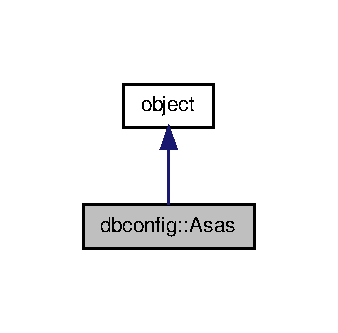
\includegraphics[width=162pt]{classdbconfig_1_1Asas__inherit__graph}
\end{center}
\end{figure}


Collaboration diagram for dbconfig::Asas:\nopagebreak
\begin{figure}[H]
\begin{center}
\leavevmode
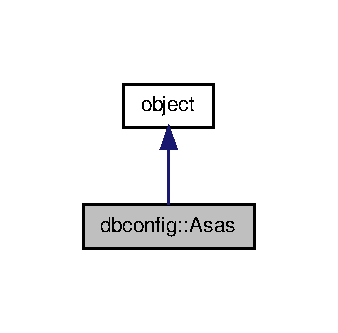
\includegraphics[width=162pt]{classdbconfig_1_1Asas__coll__graph}
\end{center}
\end{figure}
\subsection*{Public Member Functions}
\begin{DoxyCompactItemize}
\item 
def \hyperlink{classdbconfig_1_1Asas_a9c2ce09253fdd84b02778f86ac71e82f}{\_\-\_\-init\_\-\_\-}
\begin{DoxyCompactList}\small\item\em Constructor. \item\end{DoxyCompactList}\end{DoxyCompactItemize}
\subsection*{Public Attributes}
\begin{DoxyCompactItemize}
\item 
\hyperlink{classdbconfig_1_1Asas_a74b79111c0b825aada21837b4a2f63bb}{dicttname}
\item 
\hyperlink{classdbconfig_1_1Asas_a958ec28dacb03d1a14fd64e421ac6b1b}{dictcols}
\item 
\hyperlink{classdbconfig_1_1Asas_a27e982b8fa2de97613508d0f107282d0}{dicttypes}
\item 
\hyperlink{classdbconfig_1_1Asas_a785517b6dab415832015ead9bdc8ae99}{dictnulls}
\item 
\hyperlink{classdbconfig_1_1Asas_a667b865b313be2e037560d499190fae4}{npdicttype}
\item 
\hyperlink{classdbconfig_1_1Asas_af0b83fddb33f1e798d3cddf763152d87}{plctname}
\item 
\hyperlink{classdbconfig_1_1Asas_a439c8b0f83ee3f5ef8d26f32840e7b69}{plccols}
\item 
\hyperlink{classdbconfig_1_1Asas_aa821e57805b77ad50a15f22e06071bd8}{plctypes}
\item 
\hyperlink{classdbconfig_1_1Asas_a2cb6b082447d67be6147132ee3ed3a25}{plcnulls}
\item 
\hyperlink{classdbconfig_1_1Asas_ab5d570a3ba8d7ef7ad341da3ddcc20b6}{blctname}
\item 
\hyperlink{classdbconfig_1_1Asas_add840af9cc3776023edb5eec97d6bfff}{blccols}
\item 
\hyperlink{classdbconfig_1_1Asas_afbbc02c9c3a6058bb8d6ab9d28893a04}{blctypes}
\item 
\hyperlink{classdbconfig_1_1Asas_aea4e19d941bd17055de19be0cf1fc456}{blcnulls}
\item 
\hyperlink{classdbconfig_1_1Asas_af505566f2b829c8cc8a8398f971c3732}{cfftname}
\item 
\hyperlink{classdbconfig_1_1Asas_acacc892581d6c4e5b9a25c89246bd009}{cffcols}
\item 
\hyperlink{classdbconfig_1_1Asas_a9ad045c204ed1efab5a2068aaa2c6203}{cfftypes}
\item 
\hyperlink{classdbconfig_1_1Asas_a359ddb7363a0d9927d889ad9332988ab}{cffnulls}
\item 
\hyperlink{classdbconfig_1_1Asas_a3d190a817a3a3d81dbd560732dc14529}{npcoefftype}
\item 
\hyperlink{classdbconfig_1_1Asas_a6323effc0231480580e3feb140ee39cf}{fittname}
\item 
\hyperlink{classdbconfig_1_1Asas_a0557c33edf7f4d42fce873fd7114c65c}{fitcols}
\item 
\hyperlink{classdbconfig_1_1Asas_a996f14f6a823b9220977c7f2fc38f806}{fittypes}
\item 
\hyperlink{classdbconfig_1_1Asas_a71d563b5bc83e8999e1eb21fffa83ed5}{fitnulls}
\end{DoxyCompactItemize}


\subsection{Detailed Description}
class wrapper for ASAS column definitions, types etc 

Definition at line 21 of file dbconfig.py.



\subsection{Constructor \& Destructor Documentation}
\hypertarget{classdbconfig_1_1Asas_a9c2ce09253fdd84b02778f86ac71e82f}{
\index{dbconfig::Asas@{dbconfig::Asas}!\_\-\_\-init\_\-\_\-@{\_\-\_\-init\_\-\_\-}}
\index{\_\-\_\-init\_\-\_\-@{\_\-\_\-init\_\-\_\-}!dbconfig::Asas@{dbconfig::Asas}}
\subsubsection[{\_\-\_\-init\_\-\_\-}]{\setlength{\rightskip}{0pt plus 5cm}def dbconfig::Asas::\_\-\_\-init\_\-\_\- (
\begin{DoxyParamCaption}
\item[{}]{self}
\end{DoxyParamCaption}
)}}
\label{classdbconfig_1_1Asas_a9c2ce09253fdd84b02778f86ac71e82f}


Constructor. 



Definition at line 28 of file dbconfig.py.



\subsection{Member Data Documentation}
\hypertarget{classdbconfig_1_1Asas_add840af9cc3776023edb5eec97d6bfff}{
\index{dbconfig::Asas@{dbconfig::Asas}!blccols@{blccols}}
\index{blccols@{blccols}!dbconfig::Asas@{dbconfig::Asas}}
\subsubsection[{blccols}]{\setlength{\rightskip}{0pt plus 5cm}{\bf dbconfig::Asas::blccols}}}
\label{classdbconfig_1_1Asas_add840af9cc3776023edb5eec97d6bfff}


Definition at line 28 of file dbconfig.py.

\hypertarget{classdbconfig_1_1Asas_aea4e19d941bd17055de19be0cf1fc456}{
\index{dbconfig::Asas@{dbconfig::Asas}!blcnulls@{blcnulls}}
\index{blcnulls@{blcnulls}!dbconfig::Asas@{dbconfig::Asas}}
\subsubsection[{blcnulls}]{\setlength{\rightskip}{0pt plus 5cm}{\bf dbconfig::Asas::blcnulls}}}
\label{classdbconfig_1_1Asas_aea4e19d941bd17055de19be0cf1fc456}


Definition at line 28 of file dbconfig.py.

\hypertarget{classdbconfig_1_1Asas_ab5d570a3ba8d7ef7ad341da3ddcc20b6}{
\index{dbconfig::Asas@{dbconfig::Asas}!blctname@{blctname}}
\index{blctname@{blctname}!dbconfig::Asas@{dbconfig::Asas}}
\subsubsection[{blctname}]{\setlength{\rightskip}{0pt plus 5cm}{\bf dbconfig::Asas::blctname}}}
\label{classdbconfig_1_1Asas_ab5d570a3ba8d7ef7ad341da3ddcc20b6}


Definition at line 28 of file dbconfig.py.

\hypertarget{classdbconfig_1_1Asas_afbbc02c9c3a6058bb8d6ab9d28893a04}{
\index{dbconfig::Asas@{dbconfig::Asas}!blctypes@{blctypes}}
\index{blctypes@{blctypes}!dbconfig::Asas@{dbconfig::Asas}}
\subsubsection[{blctypes}]{\setlength{\rightskip}{0pt plus 5cm}{\bf dbconfig::Asas::blctypes}}}
\label{classdbconfig_1_1Asas_afbbc02c9c3a6058bb8d6ab9d28893a04}


Definition at line 28 of file dbconfig.py.

\hypertarget{classdbconfig_1_1Asas_acacc892581d6c4e5b9a25c89246bd009}{
\index{dbconfig::Asas@{dbconfig::Asas}!cffcols@{cffcols}}
\index{cffcols@{cffcols}!dbconfig::Asas@{dbconfig::Asas}}
\subsubsection[{cffcols}]{\setlength{\rightskip}{0pt plus 5cm}{\bf dbconfig::Asas::cffcols}}}
\label{classdbconfig_1_1Asas_acacc892581d6c4e5b9a25c89246bd009}


Definition at line 28 of file dbconfig.py.

\hypertarget{classdbconfig_1_1Asas_a359ddb7363a0d9927d889ad9332988ab}{
\index{dbconfig::Asas@{dbconfig::Asas}!cffnulls@{cffnulls}}
\index{cffnulls@{cffnulls}!dbconfig::Asas@{dbconfig::Asas}}
\subsubsection[{cffnulls}]{\setlength{\rightskip}{0pt plus 5cm}{\bf dbconfig::Asas::cffnulls}}}
\label{classdbconfig_1_1Asas_a359ddb7363a0d9927d889ad9332988ab}


Definition at line 28 of file dbconfig.py.

\hypertarget{classdbconfig_1_1Asas_af505566f2b829c8cc8a8398f971c3732}{
\index{dbconfig::Asas@{dbconfig::Asas}!cfftname@{cfftname}}
\index{cfftname@{cfftname}!dbconfig::Asas@{dbconfig::Asas}}
\subsubsection[{cfftname}]{\setlength{\rightskip}{0pt plus 5cm}{\bf dbconfig::Asas::cfftname}}}
\label{classdbconfig_1_1Asas_af505566f2b829c8cc8a8398f971c3732}


Definition at line 28 of file dbconfig.py.

\hypertarget{classdbconfig_1_1Asas_a9ad045c204ed1efab5a2068aaa2c6203}{
\index{dbconfig::Asas@{dbconfig::Asas}!cfftypes@{cfftypes}}
\index{cfftypes@{cfftypes}!dbconfig::Asas@{dbconfig::Asas}}
\subsubsection[{cfftypes}]{\setlength{\rightskip}{0pt plus 5cm}{\bf dbconfig::Asas::cfftypes}}}
\label{classdbconfig_1_1Asas_a9ad045c204ed1efab5a2068aaa2c6203}


Definition at line 28 of file dbconfig.py.

\hypertarget{classdbconfig_1_1Asas_a958ec28dacb03d1a14fd64e421ac6b1b}{
\index{dbconfig::Asas@{dbconfig::Asas}!dictcols@{dictcols}}
\index{dictcols@{dictcols}!dbconfig::Asas@{dbconfig::Asas}}
\subsubsection[{dictcols}]{\setlength{\rightskip}{0pt plus 5cm}{\bf dbconfig::Asas::dictcols}}}
\label{classdbconfig_1_1Asas_a958ec28dacb03d1a14fd64e421ac6b1b}


Definition at line 28 of file dbconfig.py.

\hypertarget{classdbconfig_1_1Asas_a785517b6dab415832015ead9bdc8ae99}{
\index{dbconfig::Asas@{dbconfig::Asas}!dictnulls@{dictnulls}}
\index{dictnulls@{dictnulls}!dbconfig::Asas@{dbconfig::Asas}}
\subsubsection[{dictnulls}]{\setlength{\rightskip}{0pt plus 5cm}{\bf dbconfig::Asas::dictnulls}}}
\label{classdbconfig_1_1Asas_a785517b6dab415832015ead9bdc8ae99}


Definition at line 28 of file dbconfig.py.

\hypertarget{classdbconfig_1_1Asas_a74b79111c0b825aada21837b4a2f63bb}{
\index{dbconfig::Asas@{dbconfig::Asas}!dicttname@{dicttname}}
\index{dicttname@{dicttname}!dbconfig::Asas@{dbconfig::Asas}}
\subsubsection[{dicttname}]{\setlength{\rightskip}{0pt plus 5cm}{\bf dbconfig::Asas::dicttname}}}
\label{classdbconfig_1_1Asas_a74b79111c0b825aada21837b4a2f63bb}


Definition at line 28 of file dbconfig.py.

\hypertarget{classdbconfig_1_1Asas_a27e982b8fa2de97613508d0f107282d0}{
\index{dbconfig::Asas@{dbconfig::Asas}!dicttypes@{dicttypes}}
\index{dicttypes@{dicttypes}!dbconfig::Asas@{dbconfig::Asas}}
\subsubsection[{dicttypes}]{\setlength{\rightskip}{0pt plus 5cm}{\bf dbconfig::Asas::dicttypes}}}
\label{classdbconfig_1_1Asas_a27e982b8fa2de97613508d0f107282d0}


Definition at line 28 of file dbconfig.py.

\hypertarget{classdbconfig_1_1Asas_a0557c33edf7f4d42fce873fd7114c65c}{
\index{dbconfig::Asas@{dbconfig::Asas}!fitcols@{fitcols}}
\index{fitcols@{fitcols}!dbconfig::Asas@{dbconfig::Asas}}
\subsubsection[{fitcols}]{\setlength{\rightskip}{0pt plus 5cm}{\bf dbconfig::Asas::fitcols}}}
\label{classdbconfig_1_1Asas_a0557c33edf7f4d42fce873fd7114c65c}


Definition at line 28 of file dbconfig.py.

\hypertarget{classdbconfig_1_1Asas_a71d563b5bc83e8999e1eb21fffa83ed5}{
\index{dbconfig::Asas@{dbconfig::Asas}!fitnulls@{fitnulls}}
\index{fitnulls@{fitnulls}!dbconfig::Asas@{dbconfig::Asas}}
\subsubsection[{fitnulls}]{\setlength{\rightskip}{0pt plus 5cm}{\bf dbconfig::Asas::fitnulls}}}
\label{classdbconfig_1_1Asas_a71d563b5bc83e8999e1eb21fffa83ed5}


Definition at line 28 of file dbconfig.py.

\hypertarget{classdbconfig_1_1Asas_a6323effc0231480580e3feb140ee39cf}{
\index{dbconfig::Asas@{dbconfig::Asas}!fittname@{fittname}}
\index{fittname@{fittname}!dbconfig::Asas@{dbconfig::Asas}}
\subsubsection[{fittname}]{\setlength{\rightskip}{0pt plus 5cm}{\bf dbconfig::Asas::fittname}}}
\label{classdbconfig_1_1Asas_a6323effc0231480580e3feb140ee39cf}


Definition at line 28 of file dbconfig.py.

\hypertarget{classdbconfig_1_1Asas_a996f14f6a823b9220977c7f2fc38f806}{
\index{dbconfig::Asas@{dbconfig::Asas}!fittypes@{fittypes}}
\index{fittypes@{fittypes}!dbconfig::Asas@{dbconfig::Asas}}
\subsubsection[{fittypes}]{\setlength{\rightskip}{0pt plus 5cm}{\bf dbconfig::Asas::fittypes}}}
\label{classdbconfig_1_1Asas_a996f14f6a823b9220977c7f2fc38f806}


Definition at line 28 of file dbconfig.py.

\hypertarget{classdbconfig_1_1Asas_a3d190a817a3a3d81dbd560732dc14529}{
\index{dbconfig::Asas@{dbconfig::Asas}!npcoefftype@{npcoefftype}}
\index{npcoefftype@{npcoefftype}!dbconfig::Asas@{dbconfig::Asas}}
\subsubsection[{npcoefftype}]{\setlength{\rightskip}{0pt plus 5cm}{\bf dbconfig::Asas::npcoefftype}}}
\label{classdbconfig_1_1Asas_a3d190a817a3a3d81dbd560732dc14529}


Definition at line 28 of file dbconfig.py.

\hypertarget{classdbconfig_1_1Asas_a667b865b313be2e037560d499190fae4}{
\index{dbconfig::Asas@{dbconfig::Asas}!npdicttype@{npdicttype}}
\index{npdicttype@{npdicttype}!dbconfig::Asas@{dbconfig::Asas}}
\subsubsection[{npdicttype}]{\setlength{\rightskip}{0pt plus 5cm}{\bf dbconfig::Asas::npdicttype}}}
\label{classdbconfig_1_1Asas_a667b865b313be2e037560d499190fae4}


Definition at line 28 of file dbconfig.py.

\hypertarget{classdbconfig_1_1Asas_a439c8b0f83ee3f5ef8d26f32840e7b69}{
\index{dbconfig::Asas@{dbconfig::Asas}!plccols@{plccols}}
\index{plccols@{plccols}!dbconfig::Asas@{dbconfig::Asas}}
\subsubsection[{plccols}]{\setlength{\rightskip}{0pt plus 5cm}{\bf dbconfig::Asas::plccols}}}
\label{classdbconfig_1_1Asas_a439c8b0f83ee3f5ef8d26f32840e7b69}


Definition at line 28 of file dbconfig.py.

\hypertarget{classdbconfig_1_1Asas_a2cb6b082447d67be6147132ee3ed3a25}{
\index{dbconfig::Asas@{dbconfig::Asas}!plcnulls@{plcnulls}}
\index{plcnulls@{plcnulls}!dbconfig::Asas@{dbconfig::Asas}}
\subsubsection[{plcnulls}]{\setlength{\rightskip}{0pt plus 5cm}{\bf dbconfig::Asas::plcnulls}}}
\label{classdbconfig_1_1Asas_a2cb6b082447d67be6147132ee3ed3a25}


Definition at line 28 of file dbconfig.py.

\hypertarget{classdbconfig_1_1Asas_af0b83fddb33f1e798d3cddf763152d87}{
\index{dbconfig::Asas@{dbconfig::Asas}!plctname@{plctname}}
\index{plctname@{plctname}!dbconfig::Asas@{dbconfig::Asas}}
\subsubsection[{plctname}]{\setlength{\rightskip}{0pt plus 5cm}{\bf dbconfig::Asas::plctname}}}
\label{classdbconfig_1_1Asas_af0b83fddb33f1e798d3cddf763152d87}


Definition at line 28 of file dbconfig.py.

\hypertarget{classdbconfig_1_1Asas_aa821e57805b77ad50a15f22e06071bd8}{
\index{dbconfig::Asas@{dbconfig::Asas}!plctypes@{plctypes}}
\index{plctypes@{plctypes}!dbconfig::Asas@{dbconfig::Asas}}
\subsubsection[{plctypes}]{\setlength{\rightskip}{0pt plus 5cm}{\bf dbconfig::Asas::plctypes}}}
\label{classdbconfig_1_1Asas_aa821e57805b77ad50a15f22e06071bd8}


Definition at line 28 of file dbconfig.py.



The documentation for this class was generated from the following file:\begin{DoxyCompactItemize}
\item 
src/\hyperlink{dbconfig_8py}{dbconfig.py}\end{DoxyCompactItemize}

\hypertarget{classException}{
\section{Exception Class Reference}
\label{classException}\index{Exception@{Exception}}
}


Inheritance diagram for Exception:
\nopagebreak
\begin{figure}[H]
\begin{center}
\leavevmode
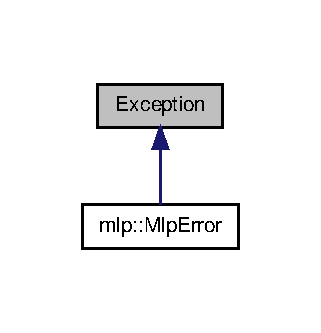
\includegraphics[width=154pt]{classException__inherit__graph}
\end{center}
\end{figure}


The documentation for this class was generated from the following file:\begin{DoxyCompactItemize}
\item 
src/\hyperlink{mlp_8py}{mlp.py}\end{DoxyCompactItemize}

\hypertarget{classmlp_1_1mlp}{
\section{mlp::mlp Class Reference}
\label{classmlp_1_1mlp}\index{mlp::mlp@{mlp::mlp}}
}


A Multi-\/Layer Perceptron.  




Inheritance diagram for mlp::mlp:\nopagebreak
\begin{figure}[H]
\begin{center}
\leavevmode
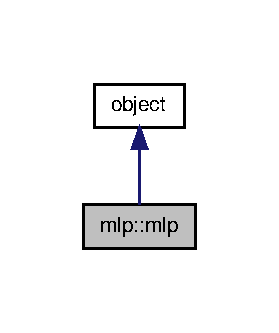
\includegraphics[width=134pt]{classmlp_1_1mlp__inherit__graph}
\end{center}
\end{figure}


Collaboration diagram for mlp::mlp:\nopagebreak
\begin{figure}[H]
\begin{center}
\leavevmode
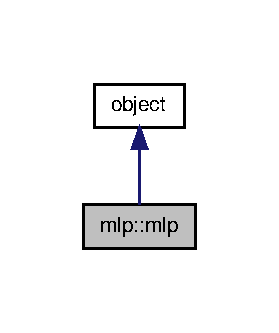
\includegraphics[width=134pt]{classmlp_1_1mlp__coll__graph}
\end{center}
\end{figure}
\subsection*{Public Member Functions}
\begin{DoxyCompactItemize}
\item 
def \hyperlink{classmlp_1_1mlp_a2bef8117288f389f454a7a96d044db73}{\_\-\_\-init\_\-\_\-}
\begin{DoxyCompactList}\small\item\em Constructor. \item\end{DoxyCompactList}\item 
def \hyperlink{classmlp_1_1mlp_a9e27c383a6bb840545bad2b0b6c18cfd}{setnormvalues}
\begin{DoxyCompactList}\small\item\em Set normalization vectors for input values: normalizedvalue = (value -\/ subtract) / devide Usually subtract is the mean value, devide the standard deviation. \item\end{DoxyCompactList}\item 
def \hyperlink{classmlp_1_1mlp_a3fadca9214b0ef2eb801f820cbe34196}{getnormvalues}
\begin{DoxyCompactList}\small\item\em Return normalization vectors. \item\end{DoxyCompactList}\item 
def \hyperlink{classmlp_1_1mlp_a8411b7d198a35a86ef134f6f7ed7045f}{setclasses}
\begin{DoxyCompactList}\small\item\em Set vector of classes. \item\end{DoxyCompactList}\item 
def \hyperlink{classmlp_1_1mlp_af3f30cb683a757eb4e9286ec48817dc4}{getclasses}
\begin{DoxyCompactList}\small\item\em Return classes network has been trained on. \item\end{DoxyCompactList}\item 
def \hyperlink{classmlp_1_1mlp_a5a681e9f1fe0aa039aa75dfb99f69f8c}{earlystopping}
\begin{DoxyCompactList}\small\item\em Train network with validation set, stop if nothing else can be learned. \item\end{DoxyCompactList}\item 
def \hyperlink{classmlp_1_1mlp_a494984c787706714539fe8f1d78efa30}{mlptrain}
\begin{DoxyCompactList}\small\item\em Train the network without validation set. \item\end{DoxyCompactList}\item 
def \hyperlink{classmlp_1_1mlp_af0925b47c421fbaeaa96dc90b0f9b6d5}{evaluate}
\begin{DoxyCompactList}\small\item\em Evaluate input values. \item\end{DoxyCompactList}\item 
def \hyperlink{classmlp_1_1mlp_a809353450c250aa532e07119c4a731ee}{confmat}
\begin{DoxyCompactList}\small\item\em Build confusion matrix. \item\end{DoxyCompactList}\item 
def \hyperlink{classmlp_1_1mlp_ad5d52821223492fb389df89622053965}{report}
\begin{DoxyCompactList}\small\item\em Print or write report of training or evaluation of inputs. \item\end{DoxyCompactList}\end{DoxyCompactItemize}
\subsection*{Public Attributes}
\begin{DoxyCompactItemize}
\item 
\hyperlink{classmlp_1_1mlp_a2769bdf0e5833e3999418868122feb28}{nin}
\item 
\hyperlink{classmlp_1_1mlp_a063008228bc8423626c2fa6e9a2664e9}{nout}
\item 
\hyperlink{classmlp_1_1mlp_a463f6e1b39fb817f6a302e522e591516}{ndata}
\item 
\hyperlink{classmlp_1_1mlp_aa34217744fa9bc0bf1e8a3b358ed0c96}{nhidden}
\item 
\hyperlink{classmlp_1_1mlp_a2f75a4b3429e0307568fc45d7e6950da}{beta}
\item 
\hyperlink{classmlp_1_1mlp_a3a4586ea27492667965ae101786a1fc8}{momentum}
\item 
\hyperlink{classmlp_1_1mlp_a1b81b434ce0227f55d266dbb4c1e03a1}{eta}
\item 
\hyperlink{classmlp_1_1mlp_a79bb54ad6f2b84903e62c0b5f5eb7344}{niterations}
\item 
\hyperlink{classmlp_1_1mlp_ad85e6054d661877c130574e54434ce16}{outtype}
\item 
\hyperlink{classmlp_1_1mlp_aa43f6dfd1707a355a974181d013e8f00}{multires}
\item 
\hyperlink{classmlp_1_1mlp_a6a417dee0a55db5f56349db1249a3ec9}{mdelta}
\item 
\hyperlink{classmlp_1_1mlp_a0573cbd708236e8af5fb46edc9c36660}{cm}
\item 
\hyperlink{classmlp_1_1mlp_a93598c8f15a234b94c33a853527bec31}{traintstats}
\item 
\hyperlink{classmlp_1_1mlp_a6ede6eef42e61e87fd2e79cf61529688}{validstats}
\item 
\hyperlink{classmlp_1_1mlp_a60e5b36a360073418d45d221ff5c47f2}{teststats}
\item 
\hyperlink{classmlp_1_1mlp_a4e81b494e111fb2c72000efbaa647963}{trainerror}
\item 
\hyperlink{classmlp_1_1mlp_a778e5d4e1b507b330dcb6804455ac416}{validerror}
\item 
\hyperlink{classmlp_1_1mlp_aa9d78571a75937654b1dbb2c78960aa1}{stopcount}
\item 
\hyperlink{classmlp_1_1mlp_aab9e6c1e9b3661fa3f276d09baf27144}{allpercent}
\item 
\hyperlink{classmlp_1_1mlp_a21e9d80982176c49feb06586010fa686}{debug}
\item 
\hyperlink{classmlp_1_1mlp_ad29044bad5109b92f57149d8bec68e14}{subdir}
\item 
\hyperlink{classmlp_1_1mlp_a07b85e2f033556b9ef42dbc9b05011c6}{writeweights}
\item 
\hyperlink{classmlp_1_1mlp_a9f1194a28bf6345709b62f34ef41a8f5}{normsubtract}
\item 
\hyperlink{classmlp_1_1mlp_a667ab65d926bd62ef896add5f059ce06}{normdevide}
\item 
\hyperlink{classmlp_1_1mlp_ae97e72b20c044203c2a86adc234eb9c5}{classes}
\item 
\hyperlink{classmlp_1_1mlp_af03c95450f5cae7754975376c0b80a66}{weights1}
\item 
\hyperlink{classmlp_1_1mlp_aab855561bd19a52513ee8b2c84facaba}{weights2}
\item 
\hyperlink{classmlp_1_1mlp_adf2a63cd452121ea5e135c191dc5723d}{trainstats}
\item 
\hyperlink{classmlp_1_1mlp_ad6d42a5405728d749f144b938b323ce1}{outputs}
\item 
\hyperlink{classmlp_1_1mlp_a4988ae34b275886fce8a1d4c6a167529}{hidden}
\end{DoxyCompactItemize}
\subsection*{Private Member Functions}
\begin{DoxyCompactItemize}
\item 
def \hyperlink{classmlp_1_1mlp_a50fab3d7313376cf2de90bcfc80db3a5}{\_\-mlpfwd}
\begin{DoxyCompactList}\small\item\em Run the network forward (internal function) \item\end{DoxyCompactList}\item 
def \hyperlink{classmlp_1_1mlp_a6adedb6cd519479a5bdec3ca7b3e0c08}{\_\-createreport}
\end{DoxyCompactItemize}


\subsection{Detailed Description}
A Multi-\/Layer Perceptron. 

Definition at line 50 of file mlp.py.



\subsection{Constructor \& Destructor Documentation}
\hypertarget{classmlp_1_1mlp_a2bef8117288f389f454a7a96d044db73}{
\index{mlp::mlp@{mlp::mlp}!\_\-\_\-init\_\-\_\-@{\_\-\_\-init\_\-\_\-}}
\index{\_\-\_\-init\_\-\_\-@{\_\-\_\-init\_\-\_\-}!mlp::mlp@{mlp::mlp}}
\subsubsection[{\_\-\_\-init\_\-\_\-}]{\setlength{\rightskip}{0pt plus 5cm}def mlp::mlp::\_\-\_\-init\_\-\_\- (
\begin{DoxyParamCaption}
\item[{}]{self, }
\item[{}]{inputs, }
\item[{}]{targets, }
\item[{}]{nhidden, }
\item[{}]{beta = {\ttfamily 1}, }
\item[{}]{momentum = {\ttfamily 0.9}, }
\item[{}]{outtype = {\ttfamily 'logistic'}, }
\item[{}]{multires = {\ttfamily False}, }
\item[{}]{mdelta = {\ttfamily 0.01}}
\end{DoxyParamCaption}
)}}
\label{classmlp_1_1mlp_a2bef8117288f389f454a7a96d044db73}


Constructor. 


\begin{DoxyParams}{Parameters}
{\em inputs} & Input values \\
\hline
{\em targets} & Target values (known classification for example) \\
\hline
{\em nhidden} & Number of neurons in hidden layer \\
\hline
{\em beta} & Scaling parameter for activation function (1.0) \\
\hline
{\em momentum} & Influence of previous learning step (0.9) \\
\hline
{\em outtype} & 'linear' or 'logistic' (default) or 'softmax' \\
\hline
{\em multires} & True if multiple results are allowed \\
\hline
{\em mdelta} & Maximum difference for a given class (0.01) \\
\hline
\end{DoxyParams}


Definition at line 64 of file mlp.py.



\subsection{Member Function Documentation}
\hypertarget{classmlp_1_1mlp_a6adedb6cd519479a5bdec3ca7b3e0c08}{
\index{mlp::mlp@{mlp::mlp}!\_\-createreport@{\_\-createreport}}
\index{\_\-createreport@{\_\-createreport}!mlp::mlp@{mlp::mlp}}
\subsubsection[{\_\-createreport}]{\setlength{\rightskip}{0pt plus 5cm}def mlp::mlp::\_\-createreport (
\begin{DoxyParamCaption}
\item[{}]{self, }
\item[{}]{classes, }
\item[{}]{titlefmt, }
\item[{}]{intfmt, }
\item[{}]{floatfmt, }
\item[{}]{firstcolfmt}
\end{DoxyParamCaption}
)\hspace{0.3cm}{\ttfamily  \mbox{[}private\mbox{]}}}}
\label{classmlp_1_1mlp_a6adedb6cd519479a5bdec3ca7b3e0c08}


Definition at line 408 of file mlp.py.

\hypertarget{classmlp_1_1mlp_a50fab3d7313376cf2de90bcfc80db3a5}{
\index{mlp::mlp@{mlp::mlp}!\_\-mlpfwd@{\_\-mlpfwd}}
\index{\_\-mlpfwd@{\_\-mlpfwd}!mlp::mlp@{mlp::mlp}}
\subsubsection[{\_\-mlpfwd}]{\setlength{\rightskip}{0pt plus 5cm}def mlp::mlp::\_\-mlpfwd (
\begin{DoxyParamCaption}
\item[{}]{self, }
\item[{}]{inputs}
\end{DoxyParamCaption}
)\hspace{0.3cm}{\ttfamily  \mbox{[}private\mbox{]}}}}
\label{classmlp_1_1mlp_a50fab3d7313376cf2de90bcfc80db3a5}


Run the network forward (internal function) 


\begin{DoxyParams}{Parameters}
{\em inputs} & Input values\\
\hline
\end{DoxyParams}
\begin{DoxyReturn}{Returns}
output Values of output layer 
\end{DoxyReturn}


Definition at line 285 of file mlp.py.

\hypertarget{classmlp_1_1mlp_a809353450c250aa532e07119c4a731ee}{
\index{mlp::mlp@{mlp::mlp}!confmat@{confmat}}
\index{confmat@{confmat}!mlp::mlp@{mlp::mlp}}
\subsubsection[{confmat}]{\setlength{\rightskip}{0pt plus 5cm}def mlp::mlp::confmat (
\begin{DoxyParamCaption}
\item[{}]{self, }
\item[{}]{inputs, }
\item[{}]{targets, }
\item[{}]{makestats = {\ttfamily True}}
\end{DoxyParamCaption}
)}}
\label{classmlp_1_1mlp_a809353450c250aa532e07119c4a731ee}


Build confusion matrix. 


\begin{DoxyParams}{Parameters}
{\em inputs} & Input values \\
\hline
{\em targets} & Target values (known classification f.e.) \\
\hline
{\em makestats} & True (default) if computing statistics for report\\
\hline
\end{DoxyParams}
\begin{DoxyReturn}{Returns}
: cm Confusion matrix 
\end{DoxyReturn}


Definition at line 354 of file mlp.py.

\hypertarget{classmlp_1_1mlp_a5a681e9f1fe0aa039aa75dfb99f69f8c}{
\index{mlp::mlp@{mlp::mlp}!earlystopping@{earlystopping}}
\index{earlystopping@{earlystopping}!mlp::mlp@{mlp::mlp}}
\subsubsection[{earlystopping}]{\setlength{\rightskip}{0pt plus 5cm}def mlp::mlp::earlystopping (
\begin{DoxyParamCaption}
\item[{}]{self, }
\item[{}]{inputs, }
\item[{}]{targets, }
\item[{}]{valid, }
\item[{}]{validtargets, }
\item[{}]{eta, }
\item[{}]{niterations = {\ttfamily 100}, }
\item[{}]{stopval = {\ttfamily 0.001}, }
\item[{}]{makestats = {\ttfamily True}}
\end{DoxyParamCaption}
)}}
\label{classmlp_1_1mlp_a5a681e9f1fe0aa039aa75dfb99f69f8c}


Train network with validation set, stop if nothing else can be learned. 

Learning stops if the validation error does falls below a limit.


\begin{DoxyParams}{Parameters}
{\em inputs} & Input values \\
\hline
{\em targets} & Target values (known classification for example) \\
\hline
{\em valid} & Validation set \\
\hline
{\em validtargets} & Target values for validation set \\
\hline
{\em eta} & Learning rate \\
\hline
{\em niterations} & Number of iterations before shuffling \\
\hline
{\em stopval} & stop at this value of validation error \\
\hline
{\em makestats} & True if statistics for report are generated (True)\\
\hline
\end{DoxyParams}
\begin{DoxyReturn}{Returns}
(validationerror, trainingerror) 
\end{DoxyReturn}


Definition at line 167 of file mlp.py.

\hypertarget{classmlp_1_1mlp_af0925b47c421fbaeaa96dc90b0f9b6d5}{
\index{mlp::mlp@{mlp::mlp}!evaluate@{evaluate}}
\index{evaluate@{evaluate}!mlp::mlp@{mlp::mlp}}
\subsubsection[{evaluate}]{\setlength{\rightskip}{0pt plus 5cm}def mlp::mlp::evaluate (
\begin{DoxyParamCaption}
\item[{}]{self, }
\item[{}]{inputs, }
\item[{}]{normalize = {\ttfamily True}}
\end{DoxyParamCaption}
)}}
\label{classmlp_1_1mlp_af0925b47c421fbaeaa96dc90b0f9b6d5}


Evaluate input values. 


\begin{DoxyParams}{Parameters}
{\em inputs} & Input values \\
\hline
{\em normalize} & True (default) if inputs should be normalized\\
\hline
\end{DoxyParams}
\begin{DoxyReturn}{Returns}
outputs Values of output layer 
\end{DoxyReturn}


Definition at line 329 of file mlp.py.

\hypertarget{classmlp_1_1mlp_af3f30cb683a757eb4e9286ec48817dc4}{
\index{mlp::mlp@{mlp::mlp}!getclasses@{getclasses}}
\index{getclasses@{getclasses}!mlp::mlp@{mlp::mlp}}
\subsubsection[{getclasses}]{\setlength{\rightskip}{0pt plus 5cm}def mlp::mlp::getclasses (
\begin{DoxyParamCaption}
\item[{}]{self}
\end{DoxyParamCaption}
)}}
\label{classmlp_1_1mlp_af3f30cb683a757eb4e9286ec48817dc4}


Return classes network has been trained on. 



Definition at line 146 of file mlp.py.

\hypertarget{classmlp_1_1mlp_a3fadca9214b0ef2eb801f820cbe34196}{
\index{mlp::mlp@{mlp::mlp}!getnormvalues@{getnormvalues}}
\index{getnormvalues@{getnormvalues}!mlp::mlp@{mlp::mlp}}
\subsubsection[{getnormvalues}]{\setlength{\rightskip}{0pt plus 5cm}def mlp::mlp::getnormvalues (
\begin{DoxyParamCaption}
\item[{}]{self}
\end{DoxyParamCaption}
)}}
\label{classmlp_1_1mlp_a3fadca9214b0ef2eb801f820cbe34196}


Return normalization vectors. 

\begin{DoxyReturn}{Returns}
(normsubtract, normdevide) 
\end{DoxyReturn}


Definition at line 128 of file mlp.py.

\hypertarget{classmlp_1_1mlp_a494984c787706714539fe8f1d78efa30}{
\index{mlp::mlp@{mlp::mlp}!mlptrain@{mlptrain}}
\index{mlptrain@{mlptrain}!mlp::mlp@{mlp::mlp}}
\subsubsection[{mlptrain}]{\setlength{\rightskip}{0pt plus 5cm}def mlp::mlp::mlptrain (
\begin{DoxyParamCaption}
\item[{}]{self, }
\item[{}]{inputs, }
\item[{}]{targets, }
\item[{}]{eta, }
\item[{}]{niterations}
\end{DoxyParamCaption}
)}}
\label{classmlp_1_1mlp_a494984c787706714539fe8f1d78efa30}


Train the network without validation set. 


\begin{DoxyParams}{Parameters}
{\em inputs} & Input values \\
\hline
{\em targets} & Target values (known classification for example) \\
\hline
{\em eta} & Learning rate \\
\hline
{\em niterations} & Number of iterations\\
\hline
\end{DoxyParams}
\begin{DoxyReturn}{Returns}
error 
\end{DoxyReturn}


Definition at line 227 of file mlp.py.

\hypertarget{classmlp_1_1mlp_ad5d52821223492fb389df89622053965}{
\index{mlp::mlp@{mlp::mlp}!report@{report}}
\index{report@{report}!mlp::mlp@{mlp::mlp}}
\subsubsection[{report}]{\setlength{\rightskip}{0pt plus 5cm}def mlp::mlp::report (
\begin{DoxyParamCaption}
\item[{}]{self, }
\item[{}]{titlefmt, }
\item[{}]{intfmt, }
\item[{}]{floatfmt, }
\item[{}]{classes = {\ttfamily None}, }
\item[{}]{ofname = {\ttfamily None}, }
\item[{}]{firstcolfmt = {\ttfamily '\%7s~'}}
\end{DoxyParamCaption}
)}}
\label{classmlp_1_1mlp_ad5d52821223492fb389df89622053965}


Print or write report of training or evaluation of inputs. 


\begin{DoxyParams}{Parameters}
{\em titlefmt,:} & Format string for class titles \\
\hline
{\em intfmt,:} & Format string for integer values \\
\hline
{\em floatfmt,:} & Format string for floating point values \\
\hline
{\em classes,:} & string with class-\/names (None = default = use self.classes) \\
\hline
{\em ofname,:} & name of output file (default = None) \\
\hline
{\em firstcolfmt,:} & Format for first columns (classes, default \char`\"{}\%7s\char`\"{}) \\
\hline
\end{DoxyParams}


Definition at line 555 of file mlp.py.

\hypertarget{classmlp_1_1mlp_a8411b7d198a35a86ef134f6f7ed7045f}{
\index{mlp::mlp@{mlp::mlp}!setclasses@{setclasses}}
\index{setclasses@{setclasses}!mlp::mlp@{mlp::mlp}}
\subsubsection[{setclasses}]{\setlength{\rightskip}{0pt plus 5cm}def mlp::mlp::setclasses (
\begin{DoxyParamCaption}
\item[{}]{self, }
\item[{}]{classes}
\end{DoxyParamCaption}
)}}
\label{classmlp_1_1mlp_a8411b7d198a35a86ef134f6f7ed7045f}


Set vector of classes. 


\begin{DoxyParams}{Parameters}
{\em classes} & String vector of classes to train on \\
\hline
\end{DoxyParams}


Definition at line 139 of file mlp.py.

\hypertarget{classmlp_1_1mlp_a9e27c383a6bb840545bad2b0b6c18cfd}{
\index{mlp::mlp@{mlp::mlp}!setnormvalues@{setnormvalues}}
\index{setnormvalues@{setnormvalues}!mlp::mlp@{mlp::mlp}}
\subsubsection[{setnormvalues}]{\setlength{\rightskip}{0pt plus 5cm}def mlp::mlp::setnormvalues (
\begin{DoxyParamCaption}
\item[{}]{self, }
\item[{}]{subtract, }
\item[{}]{devide}
\end{DoxyParamCaption}
)}}
\label{classmlp_1_1mlp_a9e27c383a6bb840545bad2b0b6c18cfd}


Set normalization vectors for input values: normalizedvalue = (value -\/ subtract) / devide Usually subtract is the mean value, devide the standard deviation. 


\begin{DoxyParams}{Parameters}
{\em subtract} & Vector of values to subtract from each input column \\
\hline
{\em devide} & Vector of values to devide difference by \\
\hline
\end{DoxyParams}


Definition at line 116 of file mlp.py.



\subsection{Member Data Documentation}
\hypertarget{classmlp_1_1mlp_aab9e6c1e9b3661fa3f276d09baf27144}{
\index{mlp::mlp@{mlp::mlp}!allpercent@{allpercent}}
\index{allpercent@{allpercent}!mlp::mlp@{mlp::mlp}}
\subsubsection[{allpercent}]{\setlength{\rightskip}{0pt plus 5cm}{\bf mlp::mlp::allpercent}}}
\label{classmlp_1_1mlp_aab9e6c1e9b3661fa3f276d09baf27144}


Definition at line 64 of file mlp.py.

\hypertarget{classmlp_1_1mlp_a2f75a4b3429e0307568fc45d7e6950da}{
\index{mlp::mlp@{mlp::mlp}!beta@{beta}}
\index{beta@{beta}!mlp::mlp@{mlp::mlp}}
\subsubsection[{beta}]{\setlength{\rightskip}{0pt plus 5cm}{\bf mlp::mlp::beta}}}
\label{classmlp_1_1mlp_a2f75a4b3429e0307568fc45d7e6950da}


Definition at line 64 of file mlp.py.

\hypertarget{classmlp_1_1mlp_ae97e72b20c044203c2a86adc234eb9c5}{
\index{mlp::mlp@{mlp::mlp}!classes@{classes}}
\index{classes@{classes}!mlp::mlp@{mlp::mlp}}
\subsubsection[{classes}]{\setlength{\rightskip}{0pt plus 5cm}{\bf mlp::mlp::classes}}}
\label{classmlp_1_1mlp_ae97e72b20c044203c2a86adc234eb9c5}


Definition at line 64 of file mlp.py.

\hypertarget{classmlp_1_1mlp_a0573cbd708236e8af5fb46edc9c36660}{
\index{mlp::mlp@{mlp::mlp}!cm@{cm}}
\index{cm@{cm}!mlp::mlp@{mlp::mlp}}
\subsubsection[{cm}]{\setlength{\rightskip}{0pt plus 5cm}{\bf mlp::mlp::cm}}}
\label{classmlp_1_1mlp_a0573cbd708236e8af5fb46edc9c36660}


Definition at line 64 of file mlp.py.

\hypertarget{classmlp_1_1mlp_a21e9d80982176c49feb06586010fa686}{
\index{mlp::mlp@{mlp::mlp}!debug@{debug}}
\index{debug@{debug}!mlp::mlp@{mlp::mlp}}
\subsubsection[{debug}]{\setlength{\rightskip}{0pt plus 5cm}{\bf mlp::mlp::debug}}}
\label{classmlp_1_1mlp_a21e9d80982176c49feb06586010fa686}


Definition at line 64 of file mlp.py.

\hypertarget{classmlp_1_1mlp_a1b81b434ce0227f55d266dbb4c1e03a1}{
\index{mlp::mlp@{mlp::mlp}!eta@{eta}}
\index{eta@{eta}!mlp::mlp@{mlp::mlp}}
\subsubsection[{eta}]{\setlength{\rightskip}{0pt plus 5cm}{\bf mlp::mlp::eta}}}
\label{classmlp_1_1mlp_a1b81b434ce0227f55d266dbb4c1e03a1}


Definition at line 64 of file mlp.py.

\hypertarget{classmlp_1_1mlp_a4988ae34b275886fce8a1d4c6a167529}{
\index{mlp::mlp@{mlp::mlp}!hidden@{hidden}}
\index{hidden@{hidden}!mlp::mlp@{mlp::mlp}}
\subsubsection[{hidden}]{\setlength{\rightskip}{0pt plus 5cm}{\bf mlp::mlp::hidden}}}
\label{classmlp_1_1mlp_a4988ae34b275886fce8a1d4c6a167529}


Definition at line 285 of file mlp.py.

\hypertarget{classmlp_1_1mlp_a6a417dee0a55db5f56349db1249a3ec9}{
\index{mlp::mlp@{mlp::mlp}!mdelta@{mdelta}}
\index{mdelta@{mdelta}!mlp::mlp@{mlp::mlp}}
\subsubsection[{mdelta}]{\setlength{\rightskip}{0pt plus 5cm}{\bf mlp::mlp::mdelta}}}
\label{classmlp_1_1mlp_a6a417dee0a55db5f56349db1249a3ec9}


Definition at line 64 of file mlp.py.

\hypertarget{classmlp_1_1mlp_a3a4586ea27492667965ae101786a1fc8}{
\index{mlp::mlp@{mlp::mlp}!momentum@{momentum}}
\index{momentum@{momentum}!mlp::mlp@{mlp::mlp}}
\subsubsection[{momentum}]{\setlength{\rightskip}{0pt plus 5cm}{\bf mlp::mlp::momentum}}}
\label{classmlp_1_1mlp_a3a4586ea27492667965ae101786a1fc8}


Definition at line 64 of file mlp.py.

\hypertarget{classmlp_1_1mlp_aa43f6dfd1707a355a974181d013e8f00}{
\index{mlp::mlp@{mlp::mlp}!multires@{multires}}
\index{multires@{multires}!mlp::mlp@{mlp::mlp}}
\subsubsection[{multires}]{\setlength{\rightskip}{0pt plus 5cm}{\bf mlp::mlp::multires}}}
\label{classmlp_1_1mlp_aa43f6dfd1707a355a974181d013e8f00}


Definition at line 64 of file mlp.py.

\hypertarget{classmlp_1_1mlp_a463f6e1b39fb817f6a302e522e591516}{
\index{mlp::mlp@{mlp::mlp}!ndata@{ndata}}
\index{ndata@{ndata}!mlp::mlp@{mlp::mlp}}
\subsubsection[{ndata}]{\setlength{\rightskip}{0pt plus 5cm}{\bf mlp::mlp::ndata}}}
\label{classmlp_1_1mlp_a463f6e1b39fb817f6a302e522e591516}


Definition at line 64 of file mlp.py.

\hypertarget{classmlp_1_1mlp_aa34217744fa9bc0bf1e8a3b358ed0c96}{
\index{mlp::mlp@{mlp::mlp}!nhidden@{nhidden}}
\index{nhidden@{nhidden}!mlp::mlp@{mlp::mlp}}
\subsubsection[{nhidden}]{\setlength{\rightskip}{0pt plus 5cm}{\bf mlp::mlp::nhidden}}}
\label{classmlp_1_1mlp_aa34217744fa9bc0bf1e8a3b358ed0c96}


Definition at line 64 of file mlp.py.

\hypertarget{classmlp_1_1mlp_a2769bdf0e5833e3999418868122feb28}{
\index{mlp::mlp@{mlp::mlp}!nin@{nin}}
\index{nin@{nin}!mlp::mlp@{mlp::mlp}}
\subsubsection[{nin}]{\setlength{\rightskip}{0pt plus 5cm}{\bf mlp::mlp::nin}}}
\label{classmlp_1_1mlp_a2769bdf0e5833e3999418868122feb28}


Definition at line 64 of file mlp.py.

\hypertarget{classmlp_1_1mlp_a79bb54ad6f2b84903e62c0b5f5eb7344}{
\index{mlp::mlp@{mlp::mlp}!niterations@{niterations}}
\index{niterations@{niterations}!mlp::mlp@{mlp::mlp}}
\subsubsection[{niterations}]{\setlength{\rightskip}{0pt plus 5cm}{\bf mlp::mlp::niterations}}}
\label{classmlp_1_1mlp_a79bb54ad6f2b84903e62c0b5f5eb7344}


Definition at line 64 of file mlp.py.

\hypertarget{classmlp_1_1mlp_a667ab65d926bd62ef896add5f059ce06}{
\index{mlp::mlp@{mlp::mlp}!normdevide@{normdevide}}
\index{normdevide@{normdevide}!mlp::mlp@{mlp::mlp}}
\subsubsection[{normdevide}]{\setlength{\rightskip}{0pt plus 5cm}{\bf mlp::mlp::normdevide}}}
\label{classmlp_1_1mlp_a667ab65d926bd62ef896add5f059ce06}


Definition at line 64 of file mlp.py.

\hypertarget{classmlp_1_1mlp_a9f1194a28bf6345709b62f34ef41a8f5}{
\index{mlp::mlp@{mlp::mlp}!normsubtract@{normsubtract}}
\index{normsubtract@{normsubtract}!mlp::mlp@{mlp::mlp}}
\subsubsection[{normsubtract}]{\setlength{\rightskip}{0pt plus 5cm}{\bf mlp::mlp::normsubtract}}}
\label{classmlp_1_1mlp_a9f1194a28bf6345709b62f34ef41a8f5}


Definition at line 64 of file mlp.py.

\hypertarget{classmlp_1_1mlp_a063008228bc8423626c2fa6e9a2664e9}{
\index{mlp::mlp@{mlp::mlp}!nout@{nout}}
\index{nout@{nout}!mlp::mlp@{mlp::mlp}}
\subsubsection[{nout}]{\setlength{\rightskip}{0pt plus 5cm}{\bf mlp::mlp::nout}}}
\label{classmlp_1_1mlp_a063008228bc8423626c2fa6e9a2664e9}


Definition at line 64 of file mlp.py.

\hypertarget{classmlp_1_1mlp_ad6d42a5405728d749f144b938b323ce1}{
\index{mlp::mlp@{mlp::mlp}!outputs@{outputs}}
\index{outputs@{outputs}!mlp::mlp@{mlp::mlp}}
\subsubsection[{outputs}]{\setlength{\rightskip}{0pt plus 5cm}{\bf mlp::mlp::outputs}}}
\label{classmlp_1_1mlp_ad6d42a5405728d749f144b938b323ce1}


Definition at line 227 of file mlp.py.

\hypertarget{classmlp_1_1mlp_ad85e6054d661877c130574e54434ce16}{
\index{mlp::mlp@{mlp::mlp}!outtype@{outtype}}
\index{outtype@{outtype}!mlp::mlp@{mlp::mlp}}
\subsubsection[{outtype}]{\setlength{\rightskip}{0pt plus 5cm}{\bf mlp::mlp::outtype}}}
\label{classmlp_1_1mlp_ad85e6054d661877c130574e54434ce16}


Definition at line 64 of file mlp.py.

\hypertarget{classmlp_1_1mlp_aa9d78571a75937654b1dbb2c78960aa1}{
\index{mlp::mlp@{mlp::mlp}!stopcount@{stopcount}}
\index{stopcount@{stopcount}!mlp::mlp@{mlp::mlp}}
\subsubsection[{stopcount}]{\setlength{\rightskip}{0pt plus 5cm}{\bf mlp::mlp::stopcount}}}
\label{classmlp_1_1mlp_aa9d78571a75937654b1dbb2c78960aa1}


Definition at line 64 of file mlp.py.

\hypertarget{classmlp_1_1mlp_ad29044bad5109b92f57149d8bec68e14}{
\index{mlp::mlp@{mlp::mlp}!subdir@{subdir}}
\index{subdir@{subdir}!mlp::mlp@{mlp::mlp}}
\subsubsection[{subdir}]{\setlength{\rightskip}{0pt plus 5cm}{\bf mlp::mlp::subdir}}}
\label{classmlp_1_1mlp_ad29044bad5109b92f57149d8bec68e14}


Definition at line 64 of file mlp.py.

\hypertarget{classmlp_1_1mlp_a60e5b36a360073418d45d221ff5c47f2}{
\index{mlp::mlp@{mlp::mlp}!teststats@{teststats}}
\index{teststats@{teststats}!mlp::mlp@{mlp::mlp}}
\subsubsection[{teststats}]{\setlength{\rightskip}{0pt plus 5cm}{\bf mlp::mlp::teststats}}}
\label{classmlp_1_1mlp_a60e5b36a360073418d45d221ff5c47f2}


Definition at line 64 of file mlp.py.

\hypertarget{classmlp_1_1mlp_a4e81b494e111fb2c72000efbaa647963}{
\index{mlp::mlp@{mlp::mlp}!trainerror@{trainerror}}
\index{trainerror@{trainerror}!mlp::mlp@{mlp::mlp}}
\subsubsection[{trainerror}]{\setlength{\rightskip}{0pt plus 5cm}{\bf mlp::mlp::trainerror}}}
\label{classmlp_1_1mlp_a4e81b494e111fb2c72000efbaa647963}


Definition at line 64 of file mlp.py.

\hypertarget{classmlp_1_1mlp_adf2a63cd452121ea5e135c191dc5723d}{
\index{mlp::mlp@{mlp::mlp}!trainstats@{trainstats}}
\index{trainstats@{trainstats}!mlp::mlp@{mlp::mlp}}
\subsubsection[{trainstats}]{\setlength{\rightskip}{0pt plus 5cm}{\bf mlp::mlp::trainstats}}}
\label{classmlp_1_1mlp_adf2a63cd452121ea5e135c191dc5723d}


Definition at line 167 of file mlp.py.

\hypertarget{classmlp_1_1mlp_a93598c8f15a234b94c33a853527bec31}{
\index{mlp::mlp@{mlp::mlp}!traintstats@{traintstats}}
\index{traintstats@{traintstats}!mlp::mlp@{mlp::mlp}}
\subsubsection[{traintstats}]{\setlength{\rightskip}{0pt plus 5cm}{\bf mlp::mlp::traintstats}}}
\label{classmlp_1_1mlp_a93598c8f15a234b94c33a853527bec31}


Definition at line 64 of file mlp.py.

\hypertarget{classmlp_1_1mlp_a778e5d4e1b507b330dcb6804455ac416}{
\index{mlp::mlp@{mlp::mlp}!validerror@{validerror}}
\index{validerror@{validerror}!mlp::mlp@{mlp::mlp}}
\subsubsection[{validerror}]{\setlength{\rightskip}{0pt plus 5cm}{\bf mlp::mlp::validerror}}}
\label{classmlp_1_1mlp_a778e5d4e1b507b330dcb6804455ac416}


Definition at line 64 of file mlp.py.

\hypertarget{classmlp_1_1mlp_a6ede6eef42e61e87fd2e79cf61529688}{
\index{mlp::mlp@{mlp::mlp}!validstats@{validstats}}
\index{validstats@{validstats}!mlp::mlp@{mlp::mlp}}
\subsubsection[{validstats}]{\setlength{\rightskip}{0pt plus 5cm}{\bf mlp::mlp::validstats}}}
\label{classmlp_1_1mlp_a6ede6eef42e61e87fd2e79cf61529688}


Definition at line 64 of file mlp.py.

\hypertarget{classmlp_1_1mlp_af03c95450f5cae7754975376c0b80a66}{
\index{mlp::mlp@{mlp::mlp}!weights1@{weights1}}
\index{weights1@{weights1}!mlp::mlp@{mlp::mlp}}
\subsubsection[{weights1}]{\setlength{\rightskip}{0pt plus 5cm}{\bf mlp::mlp::weights1}}}
\label{classmlp_1_1mlp_af03c95450f5cae7754975376c0b80a66}


Definition at line 64 of file mlp.py.

\hypertarget{classmlp_1_1mlp_aab855561bd19a52513ee8b2c84facaba}{
\index{mlp::mlp@{mlp::mlp}!weights2@{weights2}}
\index{weights2@{weights2}!mlp::mlp@{mlp::mlp}}
\subsubsection[{weights2}]{\setlength{\rightskip}{0pt plus 5cm}{\bf mlp::mlp::weights2}}}
\label{classmlp_1_1mlp_aab855561bd19a52513ee8b2c84facaba}


Definition at line 64 of file mlp.py.

\hypertarget{classmlp_1_1mlp_a07b85e2f033556b9ef42dbc9b05011c6}{
\index{mlp::mlp@{mlp::mlp}!writeweights@{writeweights}}
\index{writeweights@{writeweights}!mlp::mlp@{mlp::mlp}}
\subsubsection[{writeweights}]{\setlength{\rightskip}{0pt plus 5cm}{\bf mlp::mlp::writeweights}}}
\label{classmlp_1_1mlp_a07b85e2f033556b9ef42dbc9b05011c6}


Definition at line 64 of file mlp.py.



The documentation for this class was generated from the following file:\begin{DoxyCompactItemize}
\item 
src/\hyperlink{mlp_8py}{mlp.py}\end{DoxyCompactItemize}

\hypertarget{classmlp_1_1MlpError}{
\section{mlp::MlpError Class Reference}
\label{classmlp_1_1MlpError}\index{mlp::MlpError@{mlp::MlpError}}
}


\hyperlink{classException}{Exception} class for mlp.  




Inheritance diagram for mlp::MlpError:
\nopagebreak
\begin{figure}[H]
\begin{center}
\leavevmode
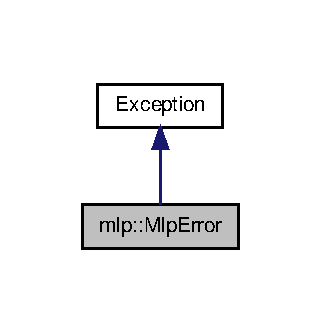
\includegraphics[width=154pt]{classmlp_1_1MlpError__inherit__graph}
\end{center}
\end{figure}


Collaboration diagram for mlp::MlpError:
\nopagebreak
\begin{figure}[H]
\begin{center}
\leavevmode
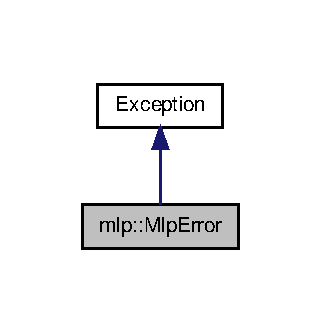
\includegraphics[width=154pt]{classmlp_1_1MlpError__coll__graph}
\end{center}
\end{figure}
\subsection*{Public Member Functions}
\begin{DoxyCompactItemize}
\item 
def \hyperlink{classmlp_1_1MlpError_a7d524593f7cdd8e23b91eba473fa9b58}{\_\-\_\-init\_\-\_\-}
\begin{DoxyCompactList}\small\item\em Constructor. \item\end{DoxyCompactList}\item 
def \hyperlink{classmlp_1_1MlpError_a660e2a1c32bf1ea08a1dcd0e123eb0be}{\_\-\_\-str\_\-\_\-}
\end{DoxyCompactItemize}
\subsection*{Public Attributes}
\begin{DoxyCompactItemize}
\item 
\hyperlink{classmlp_1_1MlpError_a2a09c605c9f8828db585739118e16f74}{value}
\end{DoxyCompactItemize}


\subsection{Detailed Description}
\hyperlink{classException}{Exception} class for mlp. 

Definition at line 28 of file mlp.py.



\subsection{Constructor \& Destructor Documentation}
\hypertarget{classmlp_1_1MlpError_a7d524593f7cdd8e23b91eba473fa9b58}{
\index{mlp::MlpError@{mlp::MlpError}!\_\-\_\-init\_\-\_\-@{\_\-\_\-init\_\-\_\-}}
\index{\_\-\_\-init\_\-\_\-@{\_\-\_\-init\_\-\_\-}!mlp::MlpError@{mlp::MlpError}}
\subsubsection[{\_\-\_\-init\_\-\_\-}]{\setlength{\rightskip}{0pt plus 5cm}def mlp::MlpError::\_\-\_\-init\_\-\_\- (
\begin{DoxyParamCaption}
\item[{}]{self, }
\item[{}]{value}
\end{DoxyParamCaption}
)}}
\label{classmlp_1_1MlpError_a7d524593f7cdd8e23b91eba473fa9b58}


Constructor. 


\begin{DoxyParams}{Parameters}
{\em value,:} & \hyperlink{classException}{Exception} value \\
\hline
\end{DoxyParams}


Definition at line 35 of file mlp.py.



\subsection{Member Function Documentation}
\hypertarget{classmlp_1_1MlpError_a660e2a1c32bf1ea08a1dcd0e123eb0be}{
\index{mlp::MlpError@{mlp::MlpError}!\_\-\_\-str\_\-\_\-@{\_\-\_\-str\_\-\_\-}}
\index{\_\-\_\-str\_\-\_\-@{\_\-\_\-str\_\-\_\-}!mlp::MlpError@{mlp::MlpError}}
\subsubsection[{\_\-\_\-str\_\-\_\-}]{\setlength{\rightskip}{0pt plus 5cm}def mlp::MlpError::\_\-\_\-str\_\-\_\- (
\begin{DoxyParamCaption}
\item[{}]{self}
\end{DoxyParamCaption}
)}}
\label{classmlp_1_1MlpError_a660e2a1c32bf1ea08a1dcd0e123eb0be}


Definition at line 39 of file mlp.py.



\subsection{Member Data Documentation}
\hypertarget{classmlp_1_1MlpError_a2a09c605c9f8828db585739118e16f74}{
\index{mlp::MlpError@{mlp::MlpError}!value@{value}}
\index{value@{value}!mlp::MlpError@{mlp::MlpError}}
\subsubsection[{value}]{\setlength{\rightskip}{0pt plus 5cm}{\bf mlp::MlpError::value}}}
\label{classmlp_1_1MlpError_a2a09c605c9f8828db585739118e16f74}


Definition at line 35 of file mlp.py.



The documentation for this class was generated from the following file:\begin{DoxyCompactItemize}
\item 
src/\hyperlink{mlp_8py}{mlp.py}\end{DoxyCompactItemize}

\hypertarget{classobject}{
\section{object Class Reference}
\label{classobject}\index{object@{object}}
}


Inheritance diagram for object:
\nopagebreak
\begin{figure}[H]
\begin{center}
\leavevmode
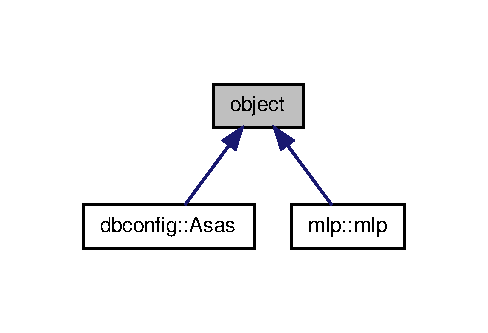
\includegraphics[width=234pt]{classobject__inherit__graph}
\end{center}
\end{figure}


The documentation for this class was generated from the following file:\begin{DoxyCompactItemize}
\item 
src/\hyperlink{mlp_8py}{mlp.py}\end{DoxyCompactItemize}

\chapter{File Documentation}
\hypertarget{dbconfig_8py}{
\section{src/dbconfig.py File Reference}
\label{dbconfig_8py}\index{src/dbconfig.py@{src/dbconfig.py}}
}
\subsection*{Classes}
\begin{DoxyCompactItemize}
\item 
class \hyperlink{classdbconfig_1_1Asas}{dbconfig::Asas}
\begin{DoxyCompactList}\small\item\em class wrapper for ASAS column definitions, types etc \item\end{DoxyCompactList}\end{DoxyCompactItemize}
\subsection*{Namespaces}
\begin{DoxyCompactItemize}
\item 
namespace \hyperlink{namespacedbconfig}{dbconfig}
\item 
namespace \hyperlink{namespaceebf}{ebf}


\begin{DoxyCompactList}\small\item\em Created on Jun 19, 2012. \item\end{DoxyCompactList}

\end{DoxyCompactItemize}

\hypertarget{functions_8py}{
\section{src/functions.py File Reference}
\label{functions_8py}\index{src/functions.py@{src/functions.py}}
}
\subsection*{Namespaces}
\begin{DoxyCompactItemize}
\item 
namespace \hyperlink{namespacefunctions}{functions}
\item 
namespace \hyperlink{namespaceebf}{ebf}


\begin{DoxyCompactList}\small\item\em Created on Jun 19, 2012. \item\end{DoxyCompactList}

\end{DoxyCompactItemize}
\subsection*{Functions}
\begin{DoxyCompactItemize}
\item 
def \hyperlink{namespacefunctions_ab417ff9b2580ed12b7937559adbc90f1}{functions::makephasedlc}
\item 
def \hyperlink{namespacefunctions_a849aa559f687aad0e0cb251f83b4dc23}{functions::deriv2}
\item 
def \hyperlink{namespacefunctions_a5cfda28c18921b966002c19c2b20b3e5}{functions::makebinnedlc}
\end{DoxyCompactItemize}

\hypertarget{makeblc_8py}{
\section{src/makeblc.py File Reference}
\label{makeblc_8py}\index{src/makeblc.py@{src/makeblc.py}}
}
\subsection*{Namespaces}
\begin{DoxyCompactItemize}
\item 
namespace \hyperlink{namespacemakeblc}{makeblc}
\item 
namespace \hyperlink{namespaceebf}{ebf}


\begin{DoxyCompactList}\small\item\em Created on Jun 19, 2012. \item\end{DoxyCompactList}

\end{DoxyCompactItemize}
\subsection*{Variables}
\begin{DoxyCompactItemize}
\item 
string \hyperlink{namespacemakeblc_af9d26964de16c4985555854c8d72580b}{makeblc::usage} = '\%prog \mbox{[}options\mbox{]} plcdbfile'
\item 
tuple \hyperlink{namespacemakeblc_a0dea09705bbc782eda44fd29626ff35b}{makeblc::parser} = OptionParser(usage=usage)
\item 
string \hyperlink{namespacemakeblc_a65838550e6d468b9df26e64e07388457}{makeblc::default} = 'asasblc.sqlite'
\item 
string \hyperlink{namespacemakeblc_a6dea7c4e16e828d56e7094476327ae97}{makeblc::help} = 'database file with phased light curves'
\item 
tuple \hyperlink{namespacemakeblc_a76c6a65c85e7590a747c0f90985c02c6}{makeblc::cls} = getattr(dbconfig, 'Asas')
\item 
tuple \hyperlink{namespacemakeblc_a69d352c98ad45dc93ce0c036904382ea}{makeblc::dbconfig} = cls()
\item 
tuple \hyperlink{namespacemakeblc_ac747659361bfa898ab3b4503fd962e9c}{makeblc::watch} = Stopwatch()
\item 
tuple \hyperlink{namespacemakeblc_a076cfa54febea93ec0a0367d9766b59b}{makeblc::dictreader} = dbr.DbReader(options.rootdir + options.dictname)
\item 
tuple \hyperlink{namespacemakeblc_a0eac396194b25b741b019161364a481e}{makeblc::generator} = dictreader.traverse(options.select, None, 1000)
\item 
int \hyperlink{namespacemakeblc_abd854e539cc9c9fe5d64b72438f277f2}{makeblc::nrstars} = 0
\item 
list \hyperlink{namespacemakeblc_aaf2dbaa320a13bde9a473d47104f7cb4}{makeblc::dictupd} = \mbox{[}$\,$\mbox{]}
\item 
tuple \hyperlink{namespacemakeblc_a0f835803cfdefeaeb151f6a83e76368f}{makeblc::plcreader} = dbr.DbReader(options.rootdir + options.plcname)
\item 
tuple \hyperlink{namespacemakeblc_aafed17d883003aa9d1b25476acf0dcb0}{makeblc::blcwriter} = dbw.DbWriter(options.rootdir + options.blcname, dbconfig.blccols)
\item 
tuple \hyperlink{namespacemakeblc_af310689cda88b823a447e448e95ee55d}{makeblc::plc} = plcreader.getlc(star\mbox{[}'uid'\mbox{]}, 'phase')
\item 
tuple \hyperlink{namespacemakeblc_a9cc6d5510f03009615ff8d73f8823bfd}{makeblc::dictwriter} = dbw.DbWriter(options.rootdir + options.dictname, dbconfig.dictcols)
\item 
string \hyperlink{namespacemakeblc_a7d13b64b84badf069728c58a2165c03d}{makeblc::updcmd} = 'update stars set fmin = ?, fmax = ?, stddev = ? where uid = ?;'
\end{DoxyCompactItemize}

\hypertarget{makeplc_8py}{\section{src/makeplc.py File Reference}
\label{makeplc_8py}\index{src/makeplc.\-py@{src/makeplc.\-py}}
}
\subsection*{Namespaces}
\begin{DoxyCompactItemize}
\item 
namespace \hyperlink{namespacemakeplc}{makeplc}
\end{DoxyCompactItemize}

\hypertarget{mlp_8py}{
\section{src/mlp.py File Reference}
\label{mlp_8py}\index{src/mlp.py@{src/mlp.py}}
}
\subsection*{Classes}
\begin{DoxyCompactItemize}
\item 
class \hyperlink{classmlp_1_1MlpError}{mlp::MlpError}
\begin{DoxyCompactList}\small\item\em \hyperlink{classException}{Exception} class for mlp. \item\end{DoxyCompactList}\item 
class \hyperlink{classmlp_1_1mlp}{mlp::mlp}
\begin{DoxyCompactList}\small\item\em A Multi-\/Layer Perceptron. \item\end{DoxyCompactList}\end{DoxyCompactItemize}
\subsection*{Namespaces}
\begin{DoxyCompactItemize}
\item 
namespace \hyperlink{namespacemlp}{mlp}
\item 
namespace \hyperlink{namespaceebf}{ebf}


\begin{DoxyCompactList}\small\item\em Created on Jun 19, 2012. \item\end{DoxyCompactList}

\end{DoxyCompactItemize}

\hypertarget{plotlc_8py}{\section{src/plotlc.py File Reference}
\label{plotlc_8py}\index{src/plotlc.\-py@{src/plotlc.\-py}}
}
\subsection*{Namespaces}
\begin{DoxyCompactItemize}
\item 
namespace \hyperlink{namespaceplotlc}{plotlc}
\end{DoxyCompactItemize}

\hypertarget{runpoly_8py}{
\section{src/runpoly.py File Reference}
\label{runpoly_8py}\index{src/runpoly.py@{src/runpoly.py}}
}
\subsection*{Namespaces}
\begin{DoxyCompactItemize}
\item 
namespace \hyperlink{namespacerunpoly}{runpoly}


\begin{DoxyCompactList}\small\item\em Created on Jul 2, 2012. \item\end{DoxyCompactList}

\end{DoxyCompactItemize}
\subsection*{Functions}
\begin{DoxyCompactItemize}
\item 
def \hyperlink{namespacerunpoly_aa4866b028ef0d94a7b9f237490073b28}{runpoly::getfit}
\item 
def \hyperlink{namespacerunpoly_a19c006c67315b888598650bbd005e703}{runpoly::fitlc}
\end{DoxyCompactItemize}
\subsection*{Variables}
\begin{DoxyCompactItemize}
\item 
string \hyperlink{namespacerunpoly_aac16bfb405f5f32d626a3c0bd057a781}{runpoly::usage} = '\%prog \mbox{[}options\mbox{]} \mbox{[}fitname\mbox{]}'
\item 
tuple \hyperlink{namespacerunpoly_a366967b50d48b6d7ab51bb4bd156ff40}{runpoly::parser} = OptionParser(usage=usage)
\item 
string \hyperlink{namespacerunpoly_afb3be1048713b880f7ac5b701514765d}{runpoly::default} = 'asasblc.sqlite'
\item 
string \hyperlink{namespacerunpoly_a7258195372f4a253f10006e02792d22b}{runpoly::help} = 'database file with binned light curves'
\item 
tuple \hyperlink{namespacerunpoly_ae53c9938e3373cc687af5896e211fcc4}{runpoly::cls} = getattr(dbconfig, 'Asas')
\item 
tuple \hyperlink{namespacerunpoly_a23238d44f53fedb2335ddfd9e0ba563a}{runpoly::dbconfig} = cls()
\item 
tuple \hyperlink{namespacerunpoly_ac9f61a81e4f1d37afe226eb29a552c68}{runpoly::tmpwriter}
\item 
tuple \hyperlink{namespacerunpoly_ac573a8d4d7a1ebbf405bd0b69fa9361b}{runpoly::watch} = Stopwatch()
\item 
tuple \hyperlink{namespacerunpoly_a41be213241b93ac1aaaf0a0dcd1818f2}{runpoly::dictreader} = dbr.DbReader(options.rootdir + options.dictname)
\item 
tuple \hyperlink{namespacerunpoly_afb96306fccc8888ba0c85e13ab7a5598}{runpoly::plcreader} = dbr.DbReader(options.rootdir + options.plcname)
\item 
tuple \hyperlink{namespacerunpoly_ac06d4b8419f2f541233264830433e74d}{runpoly::blcreader} = dbr.DbReader(options.rootdir + options.blcname)
\item 
tuple \hyperlink{namespacerunpoly_a09493fdc135109309376e8ac388a3fde}{runpoly::dictwriter}
\item 
tuple \hyperlink{namespacerunpoly_a19b081e3078cf18f986b0d40995ddd86}{runpoly::cffwriter}
\item 
tuple \hyperlink{namespacerunpoly_a270c35c20bdd6aa659cab1358e8f9475}{runpoly::fitwriter}
\item 
tuple \hyperlink{namespacerunpoly_a66f644ff5f02e8d9724a514873ac1be4}{runpoly::generator} = dictreader.traverse(options.select, None, 1000)
\item 
int \hyperlink{namespacerunpoly_aa86a45877f78f52e3357c19a9221feed}{runpoly::nrstars} = 0
\item 
int \hyperlink{namespacerunpoly_a77eea5c10faa8e40af7173ac7eda3478}{runpoly::failed} = 0
\item 
\hyperlink{namespacerunpoly_a429eb81cafed3ca14e2465cbd91d3224}{runpoly::olddir} = options.rootdir
\item 
tuple \hyperlink{namespacerunpoly_a079d0116a1dcdb50fd810307fa37f4b4}{runpoly::plc} = plcreader.getlc(star\mbox{[}'uid'\mbox{]}, 'stars', 'phase')
\item 
tuple \hyperlink{namespacerunpoly_ae215f3ab3bd79ffc8502386a8e0ca6c6}{runpoly::blc} = blcreader.getlc(star\mbox{[}'uid'\mbox{]}, 'stars', 'phase')
\end{DoxyCompactItemize}

\hypertarget{runpoly__dan__6_8py}{\section{src/runpoly\-\_\-dan\-\_\-6.py File Reference}
\label{runpoly__dan__6_8py}\index{src/runpoly\-\_\-dan\-\_\-6.\-py@{src/runpoly\-\_\-dan\-\_\-6.\-py}}
}
\subsection*{Namespaces}
\begin{DoxyCompactItemize}
\item 
namespace \hyperlink{namespacerunpoly__dan__6}{runpoly\-\_\-dan\-\_\-6}
\end{DoxyCompactItemize}

\hypertarget{runpolymp_8py}{\section{src/runpolymp.py File Reference}
\label{runpolymp_8py}\index{src/runpolymp.\-py@{src/runpolymp.\-py}}
}
\subsection*{Namespaces}
\begin{DoxyCompactItemize}
\item 
namespace \hyperlink{namespacerunpolymp}{runpolymp}
\end{DoxyCompactItemize}

\hypertarget{runtrained_8py}{\section{src/runtrained.py File Reference}
\label{runtrained_8py}\index{src/runtrained.\-py@{src/runtrained.\-py}}
}
\subsection*{Namespaces}
\begin{DoxyCompactItemize}
\item 
namespace \hyperlink{namespaceruntrained}{runtrained}
\end{DoxyCompactItemize}

\hypertarget{trainnet_8py}{
\section{src/trainnet.py File Reference}
\label{trainnet_8py}\index{src/trainnet.py@{src/trainnet.py}}
}
\subsection*{Namespaces}
\begin{DoxyCompactItemize}
\item 
namespace \hyperlink{namespacetrainnet}{trainnet}


\begin{DoxyCompactList}\small\item\em Created on Jul 5, 2012. \item\end{DoxyCompactList}

\end{DoxyCompactItemize}
\subsection*{Functions}
\begin{DoxyCompactItemize}
\item 
def \hyperlink{namespacetrainnet_af0ab122647716d110c3d20d71bca7517}{trainnet::maketarget}
\begin{DoxyCompactList}\small\item\em Set the target vector for a single object. \item\end{DoxyCompactList}\item 
def \hyperlink{namespacetrainnet_a3770060027ff2b2ac850672baaedc954}{trainnet::prepdata}
\begin{DoxyCompactList}\small\item\em Prepare data for neural network (assemble and normalize). \item\end{DoxyCompactList}\item 
def \hyperlink{namespacetrainnet_a6b2a6c6ee5f126bec6cf862ebcee3d7c}{trainnet::readdata}
\begin{DoxyCompactList}\small\item\em read data from database \item\end{DoxyCompactList}\item 
def \hyperlink{namespacetrainnet_ade5fd81c145ae647da27e5108ecbc83b}{trainnet::reshuffle}
\begin{DoxyCompactList}\small\item\em re-\/shuffling the data \item\end{DoxyCompactList}\item 
def \hyperlink{namespacetrainnet_a38102ec29b7d6d2fbf74196151247213}{trainnet::parseoptions}
\begin{DoxyCompactList}\small\item\em Parse command line options. \item\end{DoxyCompactList}\item 
def \hyperlink{namespacetrainnet_af0eeb2aa38d66cbd67256b1b27066ea4}{trainnet::splitdata}
\begin{DoxyCompactList}\small\item\em Split data into training, validation and testing set according to given fractions. \item\end{DoxyCompactList}\end{DoxyCompactItemize}
\subsection*{Variables}
\begin{DoxyCompactItemize}
\item 
tuple \hyperlink{namespacetrainnet_a92c95c206ed27e0de8dec1cb68a1f6bb}{trainnet::cls} = getattr(dbconfig, 'Asas')
\item 
tuple \hyperlink{namespacetrainnet_a293be6aa425ca070702d0f999f1ea68d}{trainnet::dbconfig} = cls()
\item 
tuple \hyperlink{namespacetrainnet_a53e6fa3504764aa1a0d61b916af6358a}{trainnet::watch} = Stopwatch()
\item 
tuple \hyperlink{namespacetrainnet_ad40ddd24354da1881bc9fe8b6547b5fa}{trainnet::watchprep} = Stopwatch()
\item 
tuple \hyperlink{namespacetrainnet_afce55f5d26936ba4b8622fc19ba56446}{trainnet::net}
\item 
\hyperlink{namespacetrainnet_a6eceefa845bebe7f22951cbc18af394b}{trainnet::eta} = options.eta,
\item 
\hyperlink{namespacetrainnet_a531ebfd51f4947ab5422381d729a8756}{trainnet::niterations} = options.nriter,
\item 
\hyperlink{namespacetrainnet_a8c0014c8c751971aa9ac67420b64d9a5}{trainnet::stopval} = options.stopval,makestatsTrue)
\item 
tuple \hyperlink{namespacetrainnet_afdfd7e6bbac45ccf3826d60cf8636299}{trainnet::cm} = net.confmat(testd, testt, True)
\item 
\hyperlink{namespacetrainnet_a3e3b093ef37c5ac35ebdcbfc08bf52e1}{trainnet::ofname} = options.repname)
\item 
tuple \hyperlink{namespacetrainnet_aacdb2e9555d0d0aa59e25c64e45d48b2}{trainnet::pf} = open(net.subdir + '/' + options.picklename, 'w')
\end{DoxyCompactItemize}

\hypertarget{trainnetmp_8py}{
\section{src/trainnetmp.py File Reference}
\label{trainnetmp_8py}\index{src/trainnetmp.py@{src/trainnetmp.py}}
}
\subsection*{Namespaces}
\begin{DoxyCompactItemize}
\item 
namespace \hyperlink{namespacetrainnetmp}{trainnetmp}


\begin{DoxyCompactList}\small\item\em Created on Jul 18, 2012. \item\end{DoxyCompactList}

\end{DoxyCompactItemize}
\subsection*{Functions}
\begin{DoxyCompactItemize}
\item 
def \hyperlink{namespacetrainnetmp_ae69cdeadf6d4d73bf96600ae218927c4}{trainnetmp::callnet}
\begin{DoxyCompactList}\small\item\em Wrapper function for calling the neural network. \item\end{DoxyCompactList}\end{DoxyCompactItemize}
\subsection*{Variables}
\begin{DoxyCompactItemize}
\item 
\hyperlink{namespacetrainnetmp_ab566ffaeaa6913a2b2b347cff1a608a4}{trainnetmp::resdir} = options.rootdir+options.resdir
\item 
\hyperlink{namespacetrainnetmp_a9ebecee08a7b0aefef2e0b192e970bda}{trainnetmp::lfname} = None
\item 
tuple \hyperlink{namespacetrainnetmp_ac6c0cf0d61312a5dbd34443a74310689}{trainnetmp::lf} = Logfile(lfname, True, True)
\item 
tuple \hyperlink{namespacetrainnetmp_ad12ea3655cd42b916f85fcedd267ad16}{trainnetmp::cls} = getattr(dbconfig, 'Asas')
\item 
tuple \hyperlink{namespacetrainnetmp_a5b13bd831f315c6820696cabf93a0d85}{trainnetmp::dbconfig} = cls()
\item 
tuple \hyperlink{namespacetrainnetmp_ad0c5cbbe64c5ef22afe865ff2f038740}{trainnetmp::watch} = Stopwatch()
\item 
tuple \hyperlink{namespacetrainnetmp_a0207abb6efd09545a76548318d6af4cf}{trainnetmp::watchprep} = Stopwatch()
\item 
tuple \hyperlink{namespacetrainnetmp_a0ce23022a012fafdc81c769f9ea2ae84}{trainnetmp::nrprocess} = int(os.environ\mbox{[}'OMP\_\-NUM\_\-THREADS'\mbox{]})
\item 
tuple \hyperlink{namespacetrainnetmp_aa0c8c776c3d1db6ced2d652b6ef39cec}{trainnetmp::args} = (traind, traint, validd, validt, options.eta, options.nriter, True)
\item 
float \hyperlink{namespacetrainnetmp_ae484804d6f3c2525ab89fc23b715d8d0}{trainnetmp::maxpercent} = 0.0
\item 
list \hyperlink{namespacetrainnetmp_acf60722e6b94f8b6613aff40c374d19f}{trainnetmp::results} = \mbox{[}$\,$\mbox{]}
\item 
tuple \hyperlink{namespacetrainnetmp_a03c784c70244aab9be7a7f087f99f1e8}{trainnetmp::pool} = Pool(processes = nrprocess)
\item 
tuple \hyperlink{namespacetrainnetmp_abc8273df12ede80d1022efecac2e6883}{trainnetmp::net}
\item 
dictionary \hyperlink{namespacetrainnetmp_afecb97f9f28c04c9cce1e3342010cd53}{trainnetmp::kwargs} = \{'net': net, 'nrhidden': i, 'iteration': j, 'logfile': lf\}
\item 
tuple \hyperlink{namespacetrainnetmp_aeaf295e503c8c7a7eb9d4e5a77ed5499}{trainnetmp::nrres} = len(results)
\item 
int \hyperlink{namespacetrainnetmp_a645db8b07923a52025222af462801dc2}{trainnetmp::oldj} = 1
\item 
float \hyperlink{namespacetrainnetmp_a8647e1123b531e4df1080e929f352389}{trainnetmp::mean} = 0.0
\item 
string \hyperlink{namespacetrainnetmp_a0fc6d0db466612f63fa6df1c682394d0}{trainnetmp::oline} = '\%2d: '
\item 
string \hyperlink{namespacetrainnetmp_a01a4fd22ee2cc1aba08b4566d95bb2a4}{trainnetmp::rname} = '/nrhidden'
\item 
tuple \hyperlink{namespacetrainnetmp_a5348e04a55d2a7563398585f1b851efa}{trainnetmp::of} = open(resdir + '/' + options.repname, 'w')
\item 
int \hyperlink{namespacetrainnetmp_aa4405feef7b967d4eb9749579d3b1dad}{trainnetmp::jmax} = 1
\item 
int \hyperlink{namespacetrainnetmp_a8c5a189bb47054d719066421ae589642}{trainnetmp::kmax} = 1
\item 
tuple \hyperlink{namespacetrainnetmp_af36e6597c6ab86263c1f5da739583e3f}{trainnetmp::cm} = net.confmat(testd, testt, True)
\item 
\hyperlink{namespacetrainnetmp_a72596b0af8ecedd242cba70b6819b03d}{trainnetmp::val} = net.allpercent
\item 
tuple \hyperlink{namespacetrainnetmp_a6b1fd4837c9650e7f0526c5e9b88fc05}{trainnetmp::pf}
\end{DoxyCompactItemize}

\printindex
\end{document}
